\documentclass[12pt,]{book}
\usepackage{lmodern}
\usepackage{amssymb,amsmath}
\usepackage{ifxetex,ifluatex}
\usepackage{fixltx2e} % provides \textsubscript
\ifnum 0\ifxetex 1\fi\ifluatex 1\fi=0 % if pdftex
  \usepackage[T1]{fontenc}
  \usepackage[utf8]{inputenc}
\else % if luatex or xelatex
  \ifxetex
    \usepackage{mathspec}
  \else
    \usepackage{fontspec}
  \fi
  \defaultfontfeatures{Ligatures=TeX,Scale=MatchLowercase}
    \setmonofont[Mapping=tex-ansi,Scale=0.7]{Source Code Pro}
\fi
% use upquote if available, for straight quotes in verbatim environments
\IfFileExists{upquote.sty}{\usepackage{upquote}}{}
% use microtype if available
\IfFileExists{microtype.sty}{%
\usepackage{microtype}
\UseMicrotypeSet[protrusion]{basicmath} % disable protrusion for tt fonts
}{}
\usepackage[margin=1in]{geometry}
\usepackage{hyperref}
\PassOptionsToPackage{usenames,dvipsnames}{color} % color is loaded by hyperref
\hypersetup{unicode=true,
            pdftitle={R Programming - Lecture Notes},
            pdfauthor={Kyun-Seop Bae},
            colorlinks=true,
            linkcolor=Maroon,
            citecolor=Blue,
            urlcolor=Blue,
            breaklinks=true}
\urlstyle{same}  % don't use monospace font for urls
\usepackage{natbib}
\bibliographystyle{apalike}
\usepackage{color}
\usepackage{fancyvrb}
\newcommand{\VerbBar}{|}
\newcommand{\VERB}{\Verb[commandchars=\\\{\}]}
\DefineVerbatimEnvironment{Highlighting}{Verbatim}{commandchars=\\\{\}}
% Add ',fontsize=\small' for more characters per line
\usepackage{framed}
\definecolor{shadecolor}{RGB}{248,248,248}
\newenvironment{Shaded}{\begin{snugshade}}{\end{snugshade}}
\newcommand{\KeywordTok}[1]{\textcolor[rgb]{0.13,0.29,0.53}{\textbf{#1}}}
\newcommand{\DataTypeTok}[1]{\textcolor[rgb]{0.13,0.29,0.53}{#1}}
\newcommand{\DecValTok}[1]{\textcolor[rgb]{0.00,0.00,0.81}{#1}}
\newcommand{\BaseNTok}[1]{\textcolor[rgb]{0.00,0.00,0.81}{#1}}
\newcommand{\FloatTok}[1]{\textcolor[rgb]{0.00,0.00,0.81}{#1}}
\newcommand{\ConstantTok}[1]{\textcolor[rgb]{0.00,0.00,0.00}{#1}}
\newcommand{\CharTok}[1]{\textcolor[rgb]{0.31,0.60,0.02}{#1}}
\newcommand{\SpecialCharTok}[1]{\textcolor[rgb]{0.00,0.00,0.00}{#1}}
\newcommand{\StringTok}[1]{\textcolor[rgb]{0.31,0.60,0.02}{#1}}
\newcommand{\VerbatimStringTok}[1]{\textcolor[rgb]{0.31,0.60,0.02}{#1}}
\newcommand{\SpecialStringTok}[1]{\textcolor[rgb]{0.31,0.60,0.02}{#1}}
\newcommand{\ImportTok}[1]{#1}
\newcommand{\CommentTok}[1]{\textcolor[rgb]{0.56,0.35,0.01}{\textit{#1}}}
\newcommand{\DocumentationTok}[1]{\textcolor[rgb]{0.56,0.35,0.01}{\textbf{\textit{#1}}}}
\newcommand{\AnnotationTok}[1]{\textcolor[rgb]{0.56,0.35,0.01}{\textbf{\textit{#1}}}}
\newcommand{\CommentVarTok}[1]{\textcolor[rgb]{0.56,0.35,0.01}{\textbf{\textit{#1}}}}
\newcommand{\OtherTok}[1]{\textcolor[rgb]{0.56,0.35,0.01}{#1}}
\newcommand{\FunctionTok}[1]{\textcolor[rgb]{0.00,0.00,0.00}{#1}}
\newcommand{\VariableTok}[1]{\textcolor[rgb]{0.00,0.00,0.00}{#1}}
\newcommand{\ControlFlowTok}[1]{\textcolor[rgb]{0.13,0.29,0.53}{\textbf{#1}}}
\newcommand{\OperatorTok}[1]{\textcolor[rgb]{0.81,0.36,0.00}{\textbf{#1}}}
\newcommand{\BuiltInTok}[1]{#1}
\newcommand{\ExtensionTok}[1]{#1}
\newcommand{\PreprocessorTok}[1]{\textcolor[rgb]{0.56,0.35,0.01}{\textit{#1}}}
\newcommand{\AttributeTok}[1]{\textcolor[rgb]{0.77,0.63,0.00}{#1}}
\newcommand{\RegionMarkerTok}[1]{#1}
\newcommand{\InformationTok}[1]{\textcolor[rgb]{0.56,0.35,0.01}{\textbf{\textit{#1}}}}
\newcommand{\WarningTok}[1]{\textcolor[rgb]{0.56,0.35,0.01}{\textbf{\textit{#1}}}}
\newcommand{\AlertTok}[1]{\textcolor[rgb]{0.94,0.16,0.16}{#1}}
\newcommand{\ErrorTok}[1]{\textcolor[rgb]{0.64,0.00,0.00}{\textbf{#1}}}
\newcommand{\NormalTok}[1]{#1}
\usepackage{longtable,booktabs}
\usepackage{graphicx,grffile}
\makeatletter
\def\maxwidth{\ifdim\Gin@nat@width>\linewidth\linewidth\else\Gin@nat@width\fi}
\def\maxheight{\ifdim\Gin@nat@height>\textheight\textheight\else\Gin@nat@height\fi}
\makeatother
% Scale images if necessary, so that they will not overflow the page
% margins by default, and it is still possible to overwrite the defaults
% using explicit options in \includegraphics[width, height, ...]{}
\setkeys{Gin}{width=\maxwidth,height=\maxheight,keepaspectratio}
\IfFileExists{parskip.sty}{%
\usepackage{parskip}
}{% else
\setlength{\parindent}{0pt}
\setlength{\parskip}{6pt plus 2pt minus 1pt}
}
\setlength{\emergencystretch}{3em}  % prevent overfull lines
\providecommand{\tightlist}{%
  \setlength{\itemsep}{0pt}\setlength{\parskip}{0pt}}
\setcounter{secnumdepth}{5}
% Redefines (sub)paragraphs to behave more like sections
\ifx\paragraph\undefined\else
\let\oldparagraph\paragraph
\renewcommand{\paragraph}[1]{\oldparagraph{#1}\mbox{}}
\fi
\ifx\subparagraph\undefined\else
\let\oldsubparagraph\subparagraph
\renewcommand{\subparagraph}[1]{\oldsubparagraph{#1}\mbox{}}
\fi

%%% Use protect on footnotes to avoid problems with footnotes in titles
\let\rmarkdownfootnote\footnote%
\def\footnote{\protect\rmarkdownfootnote}

%%% Change title format to be more compact
\usepackage{titling}

% Create subtitle command for use in maketitle
\newcommand{\subtitle}[1]{
  \posttitle{
    \begin{center}\large#1\end{center}
    }
}

\setlength{\droptitle}{-2em}
  \title{R Programming - Lecture Notes}
  \pretitle{\vspace{\droptitle}\centering\huge}
  \posttitle{\par}
  \author{Kyun-Seop Bae}
  \preauthor{\centering\large\emph}
  \postauthor{\par}
  \predate{\centering\large\emph}
  \postdate{\par}
  \date{2017-03-31}

\usepackage{kotex}
\usepackage{booktabs}
\usepackage{amsthm}
\makeatletter
\def\thm@space@setup{%
  \thm@preskip=8pt plus 2pt minus 4pt
  \thm@postskip=\thm@preskip
}
\makeatother
\newenvironment{rmdnote}
  {\begin{rmdblock}{note}}
  {\end{rmdblock}}

\begin{document}
\maketitle

{
\hypersetup{linkcolor=black}
\setcounter{tocdepth}{1}
\tableofcontents
}
\listoftables
\listoffigures
\chapter*{Preface}\label{preface}
\addcontentsline{toc}{chapter}{Preface}

안녕하십니까?

2017년 1학기 울산대학교 의학과 대학원 수업 \texttt{R\ Programming} 과목
담당교수 배균섭입니다.

R은 \url{http://cran.r-project.org} 에서 다운로드받아 설치할 수
있습니다. 역시 같은 사이트에서 Manual이 나와 있으니 참고하시기 바랍니다.
구글에서 `R Programming pdf'와 같은 키워드로 검색하시면 많은 자료를 보실
수 있습니다.

첨부한
\href{https://groups.google.com/a/acr.kr/group/r/attach/409db97bf453a/R.stx?part=0.1\&authuser=0}{R.stx}
파일은 AcroEdit이라는 editor에서 사용할 syntax highlighting용 구문
파일입니다. \url{http://www.acrosoft.pe.kr} 에서 다운로드 받아
설치하시기 바랍니다. AcroEdit대신 notepad++를 선호하시는 분은 그대로
사용하셔도 됩니다.

저는 RStudio, tinnR 등을 이용해서 강의하지 않습니다만, 필요하신 분은
쓰셔도 괜찮습니다. 향후 R package 작성을 위해서는 MiKTeX와 Rtools를
설치하십시오.

추가로 말씀드리자면, \url{http://www.coursera.org} 에 많은 R 강좌가
개설되어 있습니다. Specialization course로 들어가면 유로이지만,
(Specialization course는 여러 개의 과목이 합쳐져 있는 것입니다.) 개별
과목을 검색해서 들어가면, 무료로도 볼 수 있습니다. (대신 시험을 칠 수
없거나, certificate를 받을 수 없습니다.)

좋은 강좌가 많으니 많이 활용하시기 바립니다.

강의 장소에 불편함이 많은 것으로 생각되어, 다음과 같이 Skype 모임을
개설하였습니다. 사정상 원거리에서 오시기 불편한 분들은 활용하시기
바랍니다. 출석은 화면을 캡쳐하거나 휴대폰으로 찍은 뒤
\href{mailto:sec@acp.kr}{\nolinkurl{sec@acp.kr}},
\href{mailto:shan@acp.kr로}{\nolinkurl{shan@acp.kr로}} 보내주시면
출석으로 인정해 드립니다.

Skype 모임 참가 \url{https://meet.lync.com/uucp-acp/ksbae/SKGJ3BNQ}

2017년 3월, 배균섭 배상

The online version of this book is licensed under the
\href{http://creativecommons.org/licenses/by-nc-sa/4.0/}{Creative
Commons Attribution-NonCommercial-ShareAlike 4.0 International License}.

\begin{figure}
\centering

\includegraphics{images/by-nc-sa.png}
\caption{Creative Commons License}
\end{figure}

\section*{Teaching Assistant}\label{teaching-assistant}
\addcontentsline{toc}{section}{Teaching Assistant}

안녕하십니까? 서울아산병원 임상약리학과 전공의 한성필입니다. 수업과
관련된 여러 제반 업무를 담당하고 있습니다. 언제든 의문사항 있으면
\href{mailto:r@acr.kr}{\nolinkurl{r@acr.kr}} 로 전체 메일 보내시거나
교수님 \href{mailto:k@acr.kr}{\nolinkurl{k@acr.kr}} 혹은 제 개인 메일
\href{mailto:shan@acp.kr}{\nolinkurl{shan@acp.kr}} 로 연락해 주십시오.

교수님께서 세우신 방침에 따라 수업시간에 출석을 부르지 않을 예정입니다.
수강하시는 화면(Skype)을 휴대폰으로 사진 찍으시거나 강의실의 스크린을
사진으로 촬영하셔서 \href{mailto:sec@acp.kr}{\nolinkurl{sec@acp.kr}} /
\href{mailto:shan@acp.kr}{\nolinkurl{shan@acp.kr}} 로 동시에 보내주시면
됩니다. 가급적 ``2017-03-31 한성필 출석'' 과 같은 식의 제목을 유지해
주시면 처리하는데 큰 도움이 될 것 같습니다.

\textbf{출석 체크를 위해 전체메일을 사용하지 말아주십시오!}

아울러 수업 중에 사용한 코드/스크립트를 사용하여 R의 패키지인
\texttt{bookdown}을 사용해 웹북을 제작 중에 있습니다. \citep{R-bookdown}
여러분이 읽고 있는 이 책 자체가 R 코드의 일종인 \texttt{Rmarkdown}의
결과물이라고 보시면 됩니다.
\href{https://github.com/asancpt/Rprogramming}{Github 저장소}가 있으니
소스 코드를 보실 수 있습니다. 누구나 소스를 편집하여
\texttt{Pull\ Request}를 요청할 수 있으므로 혹시 Github를 사용하셔서
웹북의 질을 높이고자 하시는 수강생 선생님들께서는 도움을 주십시오. 혹은
웹북의 각 페이지 아래쪽에 Disqus 창을 달아놓았으므로, 궁금한 점을 메모로
남겨주셔도 좋습니다.

감사합니다.

2017년 3월, 한성필 올림

\section*{FAQ}\label{faq}
\addcontentsline{toc}{section}{FAQ}

\begin{quote}
Q. 미국학회 참석으로 수업시간이 귀국행 비행기 기내에 있을거같아 출석이
안될것 같습니다. 방법이 있을지요?
\end{quote}

결석 사유서를 제출해 주시면 출석 처리 하겠습니다.
\href{http://www.medulsan.ac.kr/graduate/?mid=72\&curpage=files}{대학원
홈페이지 참고 바랍니다.} 이 링크로 들어가시면 가장 위에 있습니다.
(\texttt{결석사유서.hwp}) 참고로 수업 영상은 녹화하여 Youtube에 비공개
링크를 만들 예정이라서 추후에 관련 영상을 시청할 수 있을 것 같습니다.
결석사유서를 제출한다고 100\% 출석이 인정되는 것은 아닙니다. 이것이
기본적으로는 offline강의이기 때문에 강의시간에 강의실에 있든지, 또는
온라인으로 접속해 있어야 합니다. 출석사유서를 제출하거나, 추후 동영상
시청을 해서 그 증거(사진)을 제출하는 경우에 감점을 줄여드릴 수 있습니다.
예를 들어, 결석시에는 2점 감점인데, 결석사유서를 제출하면 1점만
감점한다는지, 동영상을 보면 0.5점만 감점한다는지 하는 것입니다. 결석
사유서 제출 시 출석 처리 원칙에 대한 설명을 드리오니, 참고하시길
바랍니다.

\begin{quote}
Q. 스카이프를 한번도 안써봐서 이참에 사용법을 배우고있는데, 수업시작시에
상대방을 어떻게 검색해서 들어가면 될지 알려주시면 감사하겠습니다.
\end{quote}

\begin{quote}
Q. 온라인 수강시 접속하는 스카이프 주소는 무엇인지요?
\end{quote}

\url{https://meet.lync.com/uucp-acp/ksbae/SKGJ3BNQ}

Chrome 등 웹브라우저에서 위 주소를 입력하면 직접 대화방으로 연결됩니다.
(검색할 필요 없습니다.) 처음 설치시에는 Add-on이 설치될 수 있습니다.
MacOS Sierra, Win7, Win10에서 Chrome, Internet Explorer 등을 사용하여
테스트해 보았고 모두 잘 동작하였습니다. 대부분의 경우 Skype For Business
계정이 없을 것으로 생각되는데 따로 로그인할 필요 없습니다.

수업 시작 30분 전부터 대화방을 개설해 놓도록 하겠습니다.

\url{https://groups.google.com/a/acr.kr/d/msg/r/nUkrE37W2kQ/waG-FkM_BgAJ}
교수님께서 처음 보낸 메일을 참고해 주십시오.

\begin{quote}
Q. 앞으로 수업은 지난 첫수업처럼 계속 온라인 수강이 가능한 것인가요?
\end{quote}

네, 계속 온라인으로 가능합니다.

\begin{quote}
Q. 저도 웹캠을 설치하여야 하여야 하나요?
\end{quote}

설치할 필요 없습니다. 오히려 수강자의 웹캠의 전원을 꺼두시길
권고드립니다.

\begin{quote}
Q. 수강전 온라인 강의 테스트 해볼 수 있나요?
\end{quote}

수업 시작 30분 전부터 대화방을 개설하여 놓도록 하겠습니다.

\begin{quote}
Q. 과제물이 있다고 들었는데 언제 assign하게 되는지요?
\end{quote}

과제물은 빨라야 5주차 이후에 나갑니다.

\begin{quote}
Q. Coursera 강의를 듣고 증명서를 내면 출석을 얼마나 커버할 수
있을런지요?
\end{quote}

Coursera는 출석 커버보다는 grade를 올려 주기 위한 것입니다. 출석은
Skype로 커버해야 합니다. 출석의 성적 반영비율은 25\%이지만, 규정상 4회
이상 결석이면 성적이 나갈 수 없습니다.

\begin{quote}
Q. 첫 수업 때, certification 관련 말씀을 하셨는데, 정확히 coursera
사이트에서 어떤 것을 듣고, 제출을 해야하는지 궁금합니다. (비슷한 내용이
많아, 어떤것을 들어야하는지 헷갈립니다.)
\end{quote}

Coursera는 꼭 어느 것을 들어야 하는 것은 아니고, R programming과 관련된
것이라면 자유로이 골라서 들으면 됩니다. 대표적인 두 가지만 들자면 다음과
같습니다.

\begin{itemize}
\tightlist
\item
  \url{https://www.coursera.org/learn/r-programming}
\item
  \url{https://www.coursera.org/learn/r-programming-environment}
\end{itemize}

\chapter{Graphics}\label{graphics}

\begin{quote}
2017-03-22 임형석 교수님 강의
\end{quote}

R을 사용해 그림 그리는 방법에 대해 알아보겠습니다.

\section{Introduction}\label{introduction}

\begin{itemize}
\tightlist
\item
  상위수준 그림 함수는 그림을 생성한다.
\item
  하위수준 그림 함수는 기존의 그림에 그림을 추가한다.
\end{itemize}

\section{상위수준 그림 함수}\label{upper}

\subsection{상위수준 그림 함수의 주요 인자
(arguments)}\label{-----arguments}

\begin{itemize}
\tightlist
\item
  main : 제목
\item
  xlab/ylab : x축 및 y축 레이블
\item
  xlim/ylim : x축 및 y축 범위
\item
  col : 색깔
\item
  lty : 선 모양
\item
  pch : 점 모양
\item
  cex : 그림 성분의 크기
\item
  lwd : 선 굵기
\item
  type : 그림 타입
\end{itemize}

\begin{Shaded}
\begin{Highlighting}[]
\NormalTok{dta <-}\StringTok{ }\KeywordTok{read.csv}\NormalTok{(}\StringTok{"PK.csv"}\NormalTok{)}
\KeywordTok{head}\NormalTok{(dta)}
\end{Highlighting}
\end{Shaded}

\begin{verbatim}
##   ID TIME AMT    DV MDV
## 1  1 0.00   0  0.00   0
## 2  1 0.00   4  0.00   1
## 3  1 0.33   0  9.40   0
## 4  1 0.66   0 13.71   0
## 5  1 1.00   0 16.52   0
## 6  1 1.50   0 29.36   0
\end{verbatim}

\begin{Shaded}
\begin{Highlighting}[]
\KeywordTok{str}\NormalTok{(dta)}
\end{Highlighting}
\end{Shaded}

\begin{verbatim}
## 'data.frame':    456 obs. of  5 variables:
##  $ ID  : num  1 1 1 1 1 1 1 1 1 1 ...
##  $ TIME: num  0 0 0.33 0.66 1 1.5 2 3 4 6 ...
##  $ AMT : num  0 4 0 0 0 0 0 0 0 0 ...
##  $ DV  : num  0 0 9.4 13.7 16.5 ...
##  $ MDV : num  0 1 0 0 0 0 0 0 0 0 ...
\end{verbatim}

\subsection{scatter plot}\label{scatter-plot}

\begin{Shaded}
\begin{Highlighting}[]
\KeywordTok{plot}\NormalTok{(dta}\OperatorTok{$}\NormalTok{TIME[dta}\OperatorTok{$}\NormalTok{MDV}\OperatorTok{==}\DecValTok{0}\NormalTok{], dta}\OperatorTok{$}\NormalTok{DV[dta}\OperatorTok{$}\NormalTok{MDV}\OperatorTok{==}\DecValTok{0}\NormalTok{])}
\end{Highlighting}
\end{Shaded}

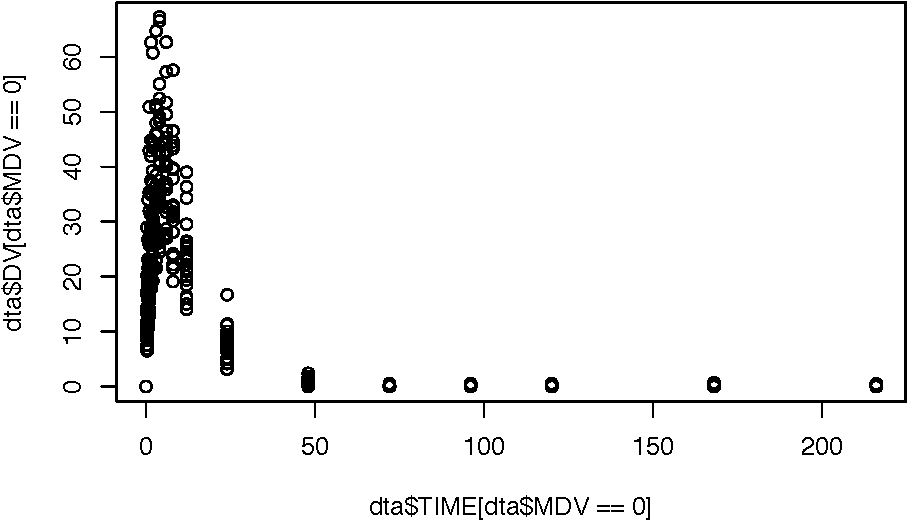
\includegraphics{Rprogramming_files/figure-latex/unnamed-chunk-3-1.pdf}

\begin{Shaded}
\begin{Highlighting}[]
\KeywordTok{plot}\NormalTok{(dta}\OperatorTok{$}\NormalTok{TIME[dta}\OperatorTok{$}\NormalTok{MDV}\OperatorTok{==}\DecValTok{0}\NormalTok{], dta}\OperatorTok{$}\NormalTok{DV[dta}\OperatorTok{$}\NormalTok{MDV}\OperatorTok{==}\DecValTok{0}\NormalTok{], }\DataTypeTok{log=}\StringTok{"y"}\NormalTok{)}
\end{Highlighting}
\end{Shaded}

\begin{verbatim}
## Warning in xy.coords(x, y, xlabel, ylabel, log): 86 y
## values <= 0 omitted from logarithmic plot
\end{verbatim}

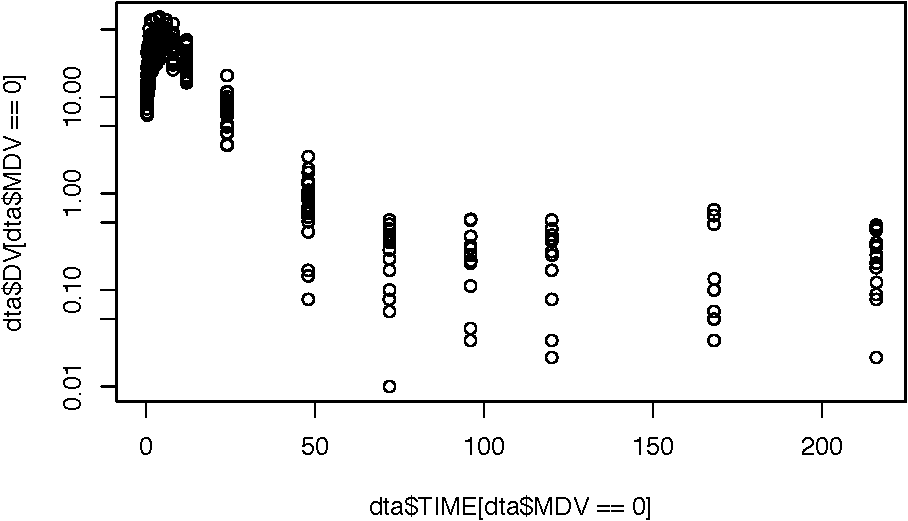
\includegraphics{Rprogramming_files/figure-latex/unnamed-chunk-3-2.pdf}

\begin{Shaded}
\begin{Highlighting}[]
\KeywordTok{plot}\NormalTok{(dta}\OperatorTok{$}\NormalTok{TIME[dta}\OperatorTok{$}\NormalTok{MDV}\OperatorTok{==}\DecValTok{0}\NormalTok{], }\KeywordTok{log}\NormalTok{(dta}\OperatorTok{$}\NormalTok{DV[dta}\OperatorTok{$}\NormalTok{MDV}\OperatorTok{==}\DecValTok{0}\NormalTok{]))}
\end{Highlighting}
\end{Shaded}

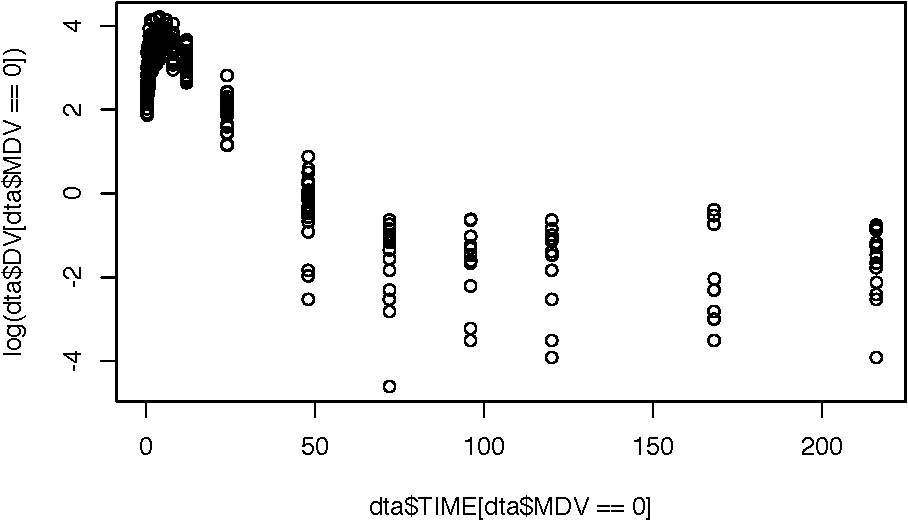
\includegraphics{Rprogramming_files/figure-latex/unnamed-chunk-3-3.pdf}

\begin{Shaded}
\begin{Highlighting}[]
\KeywordTok{plot}\NormalTok{(dta}\OperatorTok{$}\NormalTok{TIME[dta}\OperatorTok{$}\NormalTok{MDV}\OperatorTok{==}\DecValTok{0}\NormalTok{], dta}\OperatorTok{$}\NormalTok{DV[dta}\OperatorTok{$}\NormalTok{MDV}\OperatorTok{==}\DecValTok{0}\NormalTok{]}
\NormalTok{     , }\DataTypeTok{xlab=}\StringTok{"Time (hr)"}\NormalTok{, }\DataTypeTok{ylab=}\StringTok{"Concentration (ng/mL)"} 
\NormalTok{     , }\DataTypeTok{type=}\StringTok{"o"}\NormalTok{, }\DataTypeTok{pch=}\DecValTok{2}\NormalTok{, }\DataTypeTok{col=}\DecValTok{1}\NormalTok{, }\DataTypeTok{main=}\StringTok{"PK time-course of Drug X"}
\NormalTok{     , }\DataTypeTok{xlim =}\KeywordTok{c}\NormalTok{(}\OperatorTok{-}\DecValTok{2}\NormalTok{,}\DecValTok{218}\NormalTok{), }\DataTypeTok{ylim=}\KeywordTok{c}\NormalTok{(}\DecValTok{0}\NormalTok{,}\DecValTok{80}\NormalTok{))}
\end{Highlighting}
\end{Shaded}

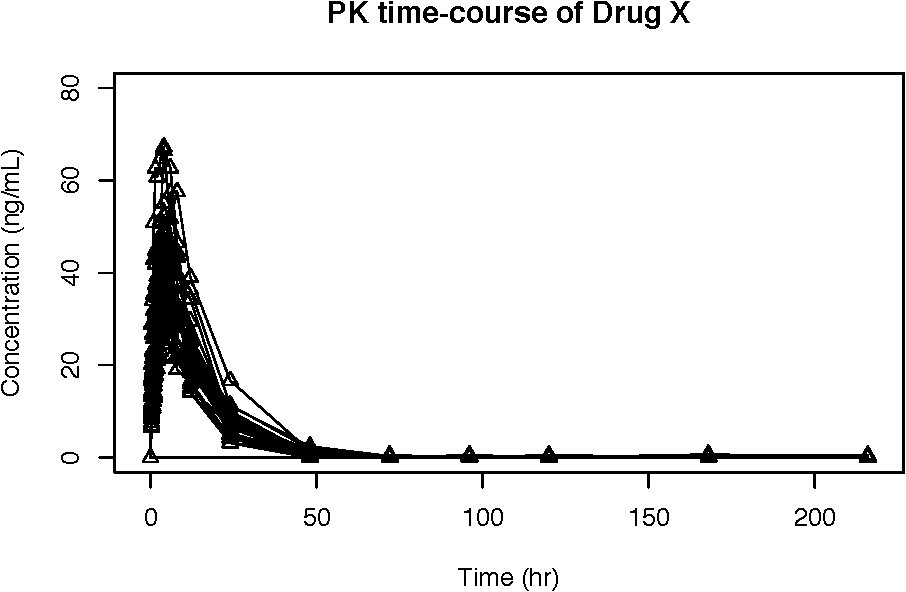
\includegraphics{Rprogramming_files/figure-latex/unnamed-chunk-3-4.pdf}

\begin{Shaded}
\begin{Highlighting}[]
\KeywordTok{plot}\NormalTok{(dta}\OperatorTok{$}\NormalTok{TIME[dta}\OperatorTok{$}\NormalTok{MDV}\OperatorTok{==}\DecValTok{0}\NormalTok{], dta}\OperatorTok{$}\NormalTok{DV[dta}\OperatorTok{$}\NormalTok{MDV}\OperatorTok{==}\DecValTok{0}\NormalTok{], }\DataTypeTok{axes=}\NormalTok{F,}
\NormalTok{     , }\DataTypeTok{xlab=}\StringTok{"Time (hr)"}\NormalTok{, }\DataTypeTok{ylab=}\StringTok{"Concentration (ng/mL)"} 
\NormalTok{     , }\DataTypeTok{type=}\StringTok{"o"}\NormalTok{, }\DataTypeTok{pch=}\DecValTok{2}\NormalTok{, }\DataTypeTok{col=}\DecValTok{1}\NormalTok{, }\DataTypeTok{main=}\StringTok{"PK time-course of Drug X"}
\NormalTok{     , }\DataTypeTok{xlim =}\KeywordTok{c}\NormalTok{(}\OperatorTok{-}\DecValTok{2}\NormalTok{,}\DecValTok{218}\NormalTok{), }\DataTypeTok{ylim=}\KeywordTok{c}\NormalTok{(}\DecValTok{0}\NormalTok{,}\DecValTok{80}\NormalTok{))}
\KeywordTok{axis}\NormalTok{(}\DecValTok{1}\NormalTok{, }\DataTypeTok{at=}\KeywordTok{seq}\NormalTok{(}\DecValTok{0}\NormalTok{, }\DecValTok{218}\NormalTok{, }\DecValTok{24}\NormalTok{))}
\KeywordTok{axis}\NormalTok{(}\DecValTok{2}\NormalTok{)}
\KeywordTok{box}\NormalTok{()}
\end{Highlighting}
\end{Shaded}

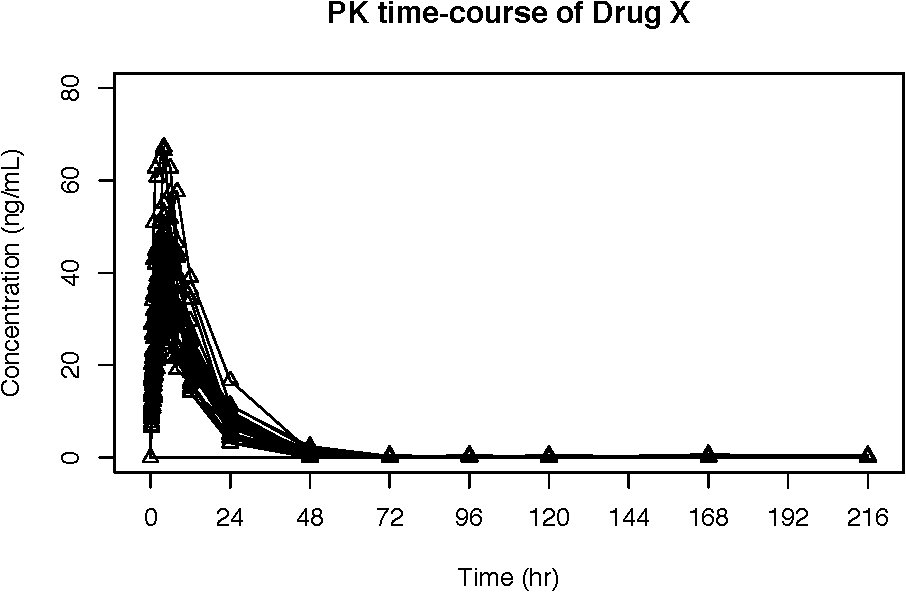
\includegraphics{Rprogramming_files/figure-latex/unnamed-chunk-3-5.pdf}

\subsection{Histogram}\label{histogram}

\begin{Shaded}
\begin{Highlighting}[]
\NormalTok{d.demog <-}\StringTok{ }\KeywordTok{read.csv}\NormalTok{(}\StringTok{"DEMOG.csv"}\NormalTok{)}

\KeywordTok{hist}\NormalTok{(d.demog}\OperatorTok{$}\NormalTok{HT)}
\end{Highlighting}
\end{Shaded}

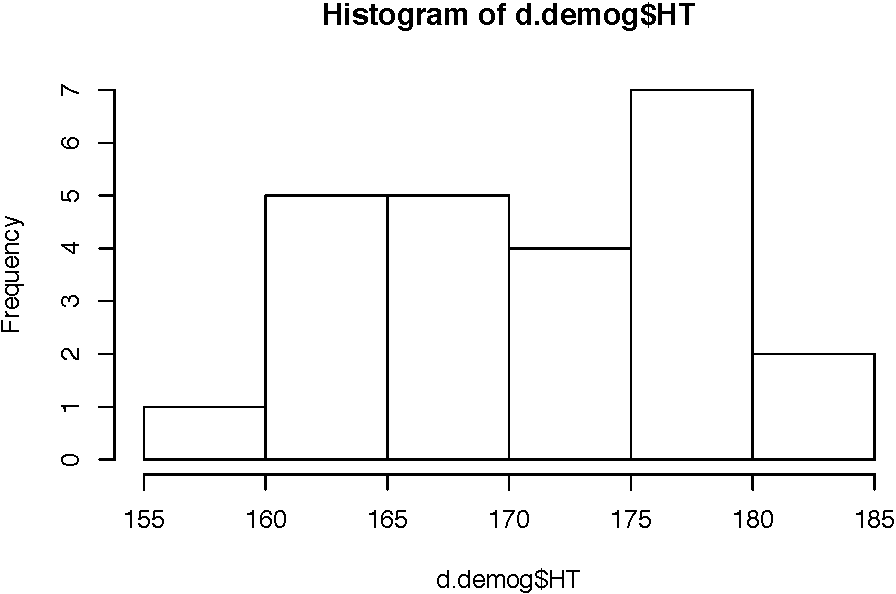
\includegraphics{Rprogramming_files/figure-latex/unnamed-chunk-4-1.pdf}

\begin{Shaded}
\begin{Highlighting}[]
\KeywordTok{hist}\NormalTok{(d.demog}\OperatorTok{$}\NormalTok{HT, }\DataTypeTok{breaks=}\DecValTok{10}\NormalTok{)}
\KeywordTok{hist}\NormalTok{(d.demog}\OperatorTok{$}\NormalTok{HT, }\DataTypeTok{nclass=}\DecValTok{10}\NormalTok{)}
\end{Highlighting}
\end{Shaded}

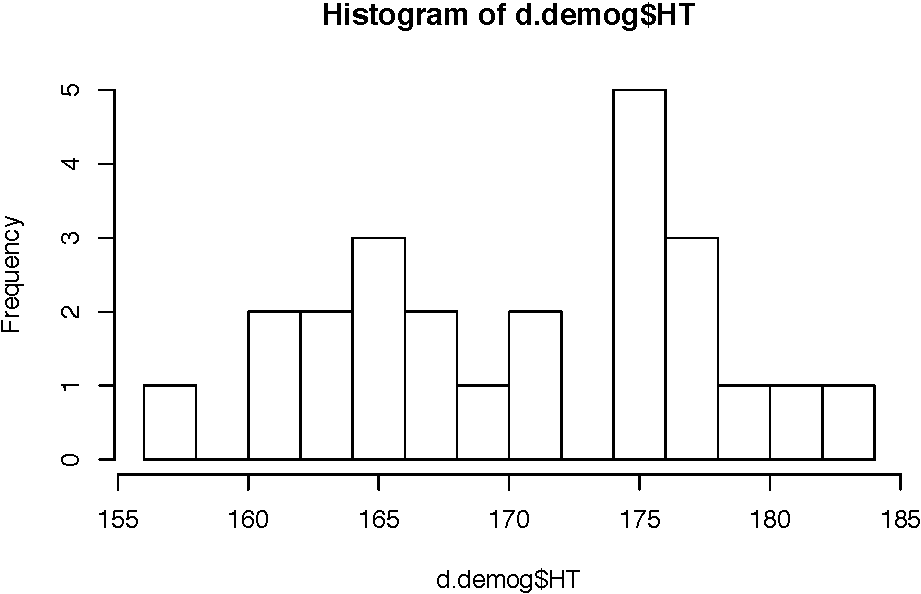
\includegraphics{Rprogramming_files/figure-latex/unnamed-chunk-4-2.pdf}

\subsubsection{with density line}\label{with-density-line}

\begin{Shaded}
\begin{Highlighting}[]
\KeywordTok{hist}\NormalTok{ (d.demog}\OperatorTok{$}\NormalTok{HT, }\DataTypeTok{probability=}\OtherTok{TRUE}\NormalTok{, }\DataTypeTok{breaks=}\DecValTok{10}\NormalTok{)}
\KeywordTok{lines}\NormalTok{(}\KeywordTok{density}\NormalTok{(d.demog}\OperatorTok{$}\NormalTok{HT))}
\end{Highlighting}
\end{Shaded}

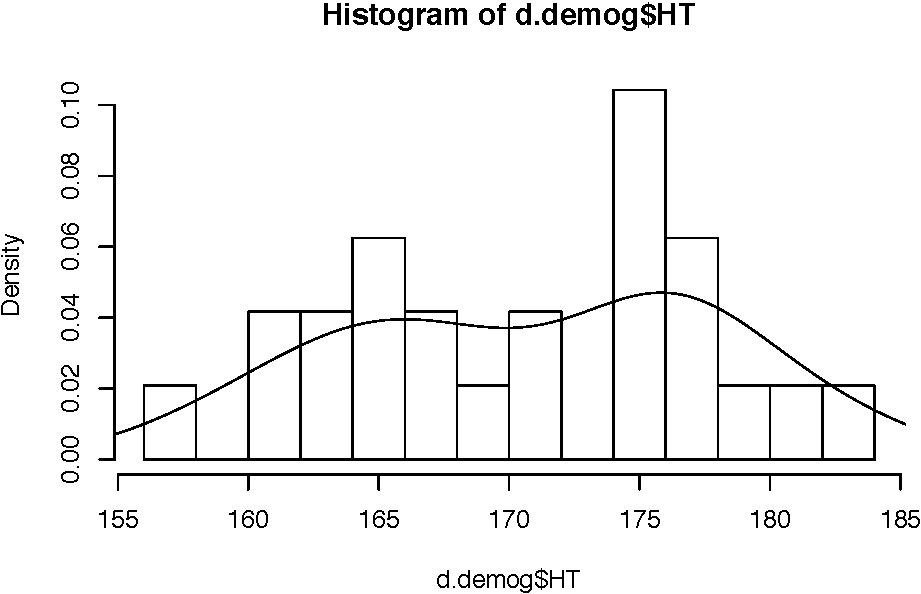
\includegraphics{Rprogramming_files/figure-latex/unnamed-chunk-5-1.pdf}

\begin{Shaded}
\begin{Highlighting}[]
\KeywordTok{hist}\NormalTok{ (d.demog}\OperatorTok{$}\NormalTok{HT, }\DataTypeTok{probability=}\OtherTok{TRUE}\NormalTok{, }\DataTypeTok{breaks=}\DecValTok{9}\NormalTok{, }\DataTypeTok{xaxt=}\StringTok{"n"}
\NormalTok{      , }\DataTypeTok{main=}\StringTok{"Histogram for Height"}\NormalTok{, }\DataTypeTok{xlab=}\StringTok{"Height (cm)"}\NormalTok{, }\DataTypeTok{ylab=}\StringTok{"Probability (%)"}\NormalTok{)}
\KeywordTok{axis}\NormalTok{(}\DecValTok{1}\NormalTok{, }\DataTypeTok{at=}\KeywordTok{seq}\NormalTok{(}\KeywordTok{min}\NormalTok{(d.demog}\OperatorTok{$}\NormalTok{HT), }\KeywordTok{max}\NormalTok{(d.demog}\OperatorTok{$}\NormalTok{HT), }\DecValTok{3}\NormalTok{))}
\KeywordTok{lines}\NormalTok{(}\KeywordTok{density}\NormalTok{(d.demog}\OperatorTok{$}\NormalTok{HT))}
\end{Highlighting}
\end{Shaded}

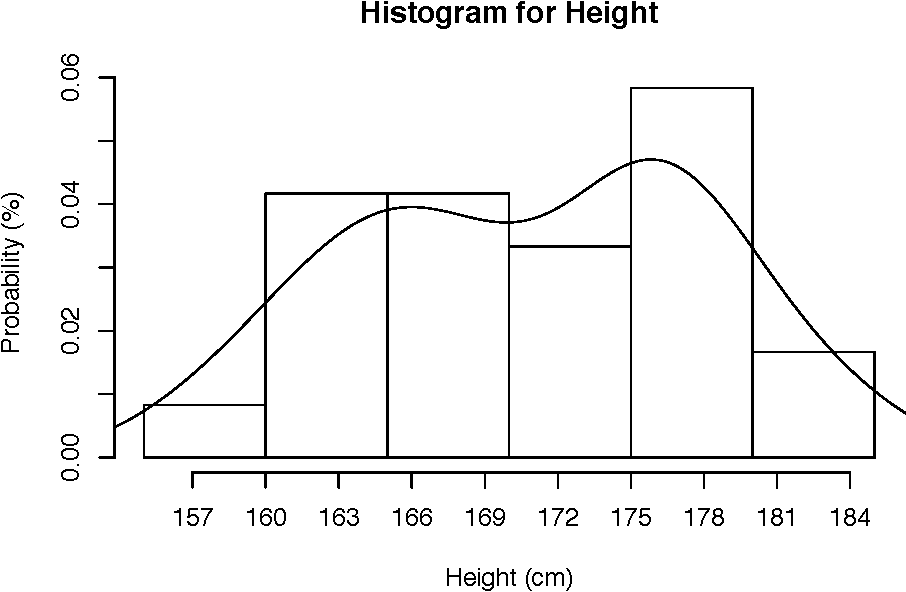
\includegraphics{Rprogramming_files/figure-latex/unnamed-chunk-5-2.pdf}

\begin{Shaded}
\begin{Highlighting}[]
\KeywordTok{hist}\NormalTok{ (d.demog}\OperatorTok{$}\NormalTok{HT, }\DataTypeTok{probability=}\OtherTok{TRUE}\NormalTok{, }\DataTypeTok{breaks=}\DecValTok{9}\NormalTok{, }\DataTypeTok{xaxt=}\StringTok{"n"}
\NormalTok{      , }\DataTypeTok{main=}\StringTok{"Histogram for Height"}\NormalTok{, }\DataTypeTok{xlab=}\StringTok{"Height (cm)"}\NormalTok{, }\DataTypeTok{ylab=}\StringTok{"Probability (%)"}
\NormalTok{      , }\DataTypeTok{col =} \StringTok{"lightblue"}\NormalTok{, }\DataTypeTok{border =} \StringTok{"pink"}\NormalTok{)}
\KeywordTok{axis}\NormalTok{(}\DecValTok{1}\NormalTok{, }\DataTypeTok{at=}\KeywordTok{seq}\NormalTok{(}\KeywordTok{min}\NormalTok{(d.demog}\OperatorTok{$}\NormalTok{HT), }\KeywordTok{max}\NormalTok{(d.demog}\OperatorTok{$}\NormalTok{HT), }\DecValTok{3}\NormalTok{))}
\KeywordTok{lines}\NormalTok{(}\KeywordTok{density}\NormalTok{(d.demog}\OperatorTok{$}\NormalTok{HT))}
\end{Highlighting}
\end{Shaded}

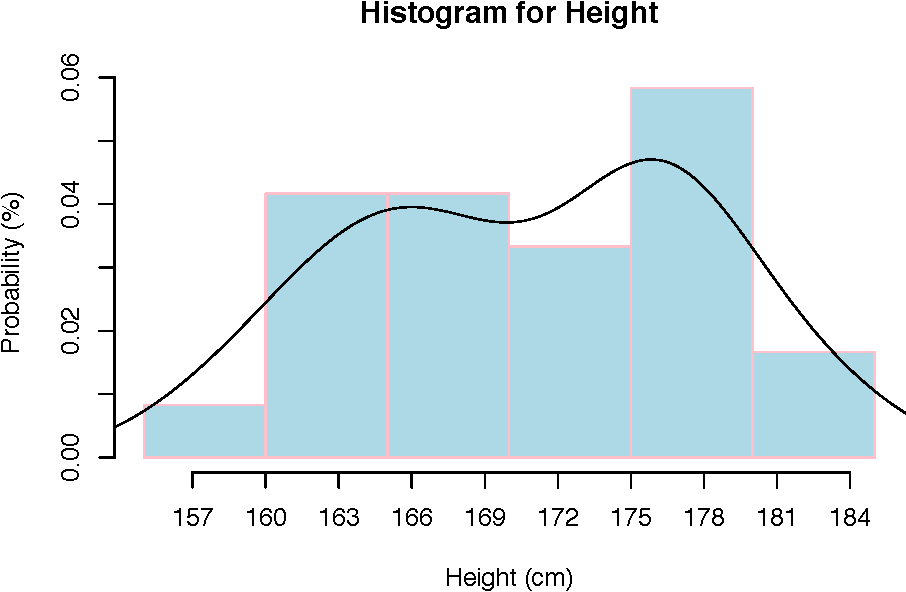
\includegraphics{Rprogramming_files/figure-latex/unnamed-chunk-5-3.pdf}

\subsection{Box-Whisker Plot}\label{box-whisker-plot}

\begin{Shaded}
\begin{Highlighting}[]
\KeywordTok{boxplot}\NormalTok{(d.demog}\OperatorTok{$}\NormalTok{WT)}
\end{Highlighting}
\end{Shaded}

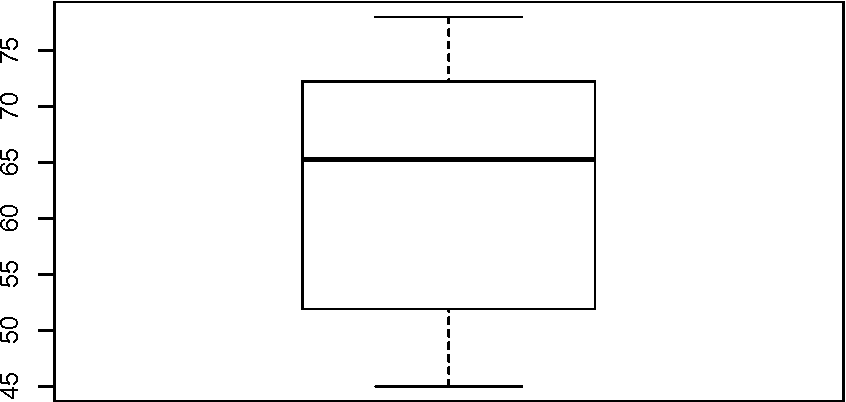
\includegraphics{Rprogramming_files/figure-latex/unnamed-chunk-6-1.pdf}

\begin{Shaded}
\begin{Highlighting}[]
\KeywordTok{boxplot}\NormalTok{(d.demog}\OperatorTok{$}\NormalTok{WT }\OperatorTok{~}\StringTok{ }\NormalTok{d.demog}\OperatorTok{$}\NormalTok{SEX)}

\KeywordTok{boxplot}\NormalTok{(}\KeywordTok{split}\NormalTok{(d.demog}\OperatorTok{$}\NormalTok{WT, d.demog}\OperatorTok{$}\NormalTok{SEX))}
\end{Highlighting}
\end{Shaded}

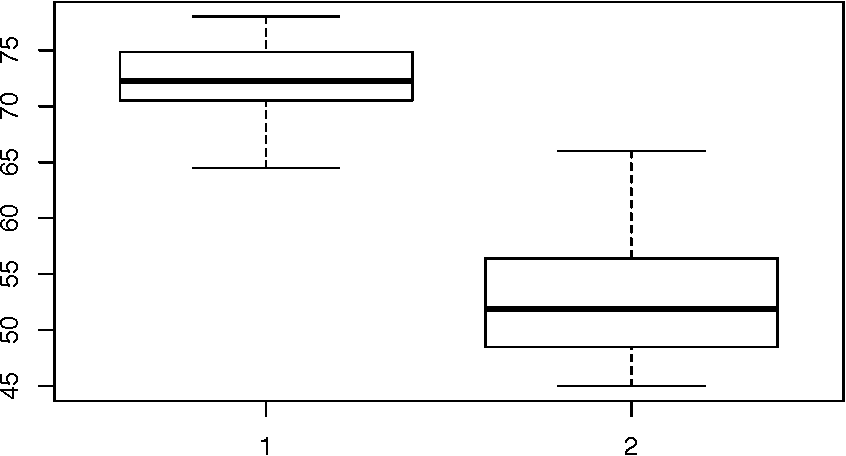
\includegraphics{Rprogramming_files/figure-latex/unnamed-chunk-6-2.pdf}

\begin{Shaded}
\begin{Highlighting}[]
\KeywordTok{boxplot}\NormalTok{(WT }\OperatorTok{~}\StringTok{ }\NormalTok{SEX, }\DataTypeTok{data=}\NormalTok{d.demog)}

\KeywordTok{boxplot}\NormalTok{(d.demog}\OperatorTok{$}\NormalTok{WT }\OperatorTok{~}\StringTok{ }\NormalTok{d.demog}\OperatorTok{$}\NormalTok{SEX}
\NormalTok{        , }\DataTypeTok{names=}\KeywordTok{c}\NormalTok{(}\StringTok{"Male"}\NormalTok{,}\StringTok{"Female"}\NormalTok{), }\DataTypeTok{ylab=}\StringTok{"AGE, year"}\NormalTok{, }\DataTypeTok{ylim=}\KeywordTok{c}\NormalTok{(}\KeywordTok{min}\NormalTok{(d.demog}\OperatorTok{$}\NormalTok{WT)}\OperatorTok{-}\DecValTok{2}\NormalTok{, }\KeywordTok{max}\NormalTok{(d.demog}\OperatorTok{$}\NormalTok{WT)}\OperatorTok{+}\DecValTok{2}\NormalTok{)}
\NormalTok{        , }\DataTypeTok{col=}\StringTok{"pink"}\NormalTok{)}
\end{Highlighting}
\end{Shaded}

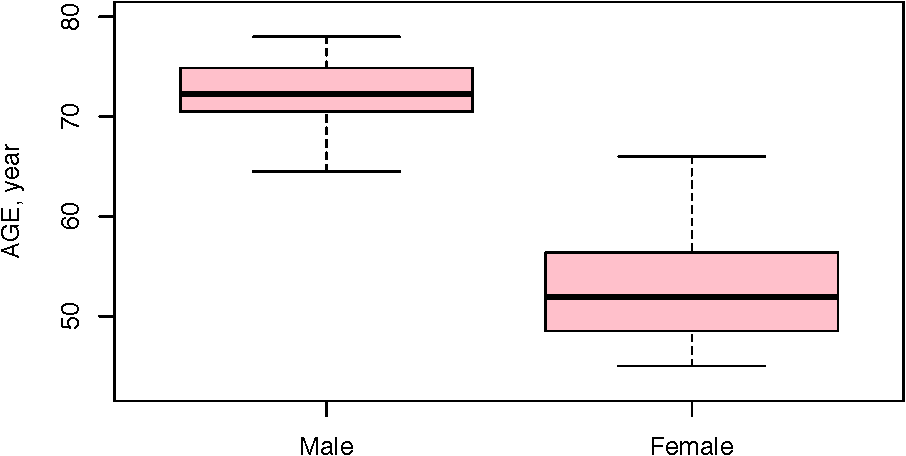
\includegraphics{Rprogramming_files/figure-latex/unnamed-chunk-6-3.pdf}

\begin{Shaded}
\begin{Highlighting}[]
\KeywordTok{boxplot}\NormalTok{(d.demog}\OperatorTok{$}\NormalTok{WT }\OperatorTok{~}\StringTok{ }\NormalTok{d.demog}\OperatorTok{$}\NormalTok{SEX}
\NormalTok{        , }\DataTypeTok{names=}\KeywordTok{c}\NormalTok{(}\StringTok{"Male"}\NormalTok{,}\StringTok{"Female"}\NormalTok{), }\DataTypeTok{ylab=}\StringTok{"AGE, year"}\NormalTok{, }\DataTypeTok{ylim=}\KeywordTok{c}\NormalTok{(}\KeywordTok{min}\NormalTok{(d.demog}\OperatorTok{$}\NormalTok{WT)}\OperatorTok{-}\DecValTok{2}\NormalTok{, }\KeywordTok{max}\NormalTok{(d.demog}\OperatorTok{$}\NormalTok{WT)}\OperatorTok{+}\DecValTok{2}\NormalTok{)}
\NormalTok{        , }\DataTypeTok{col=}\KeywordTok{c}\NormalTok{(}\StringTok{"lightblue"}\NormalTok{, }\StringTok{"salmon"}\NormalTok{), }\DataTypeTok{width=}\KeywordTok{c}\NormalTok{(}\FloatTok{0.6}\NormalTok{, }\DecValTok{1}\NormalTok{))}
\end{Highlighting}
\end{Shaded}

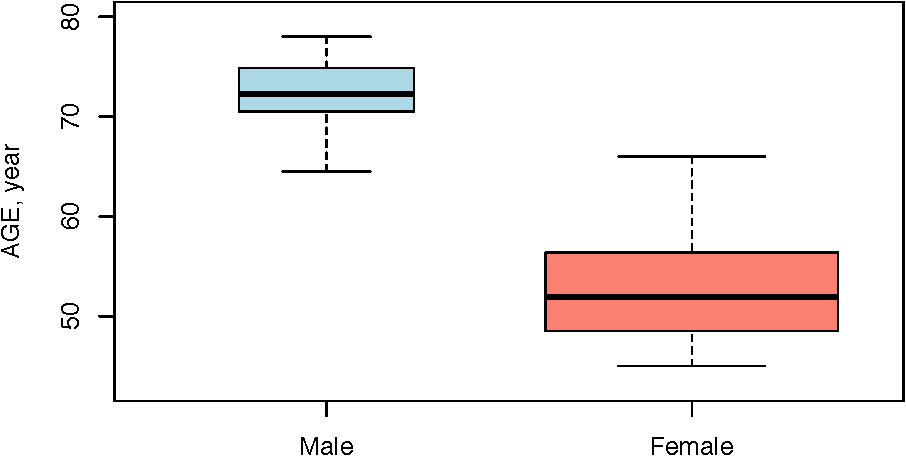
\includegraphics{Rprogramming_files/figure-latex/unnamed-chunk-6-4.pdf}

-varwidth: if varwidth is TRUE, the boxes are drawn with widths
proportional to the square-roots of the number of observations in the
groups.

\begin{Shaded}
\begin{Highlighting}[]
\KeywordTok{boxplot}\NormalTok{(d.demog}\OperatorTok{$}\NormalTok{WT }\OperatorTok{~}\StringTok{ }\NormalTok{d.demog}\OperatorTok{$}\NormalTok{SEX}
\NormalTok{        , }\DataTypeTok{names=}\KeywordTok{c}\NormalTok{(}\StringTok{"Male"}\NormalTok{,}\StringTok{"Female"}\NormalTok{), }\DataTypeTok{ylab=}\StringTok{"AGE, year"}\NormalTok{, }\DataTypeTok{ylim=}\KeywordTok{c}\NormalTok{(}\KeywordTok{min}\NormalTok{(d.demog}\OperatorTok{$}\NormalTok{WT)}\OperatorTok{-}\DecValTok{2}\NormalTok{, }\KeywordTok{max}\NormalTok{(d.demog}\OperatorTok{$}\NormalTok{WT)}\OperatorTok{+}\DecValTok{2}\NormalTok{)}
\NormalTok{        , }\DataTypeTok{col=}\KeywordTok{c}\NormalTok{(}\StringTok{"lightblue"}\NormalTok{, }\StringTok{"salmon"}\NormalTok{)}
\NormalTok{        , }\DataTypeTok{varwidth=}\OtherTok{TRUE}\NormalTok{)}
\end{Highlighting}
\end{Shaded}

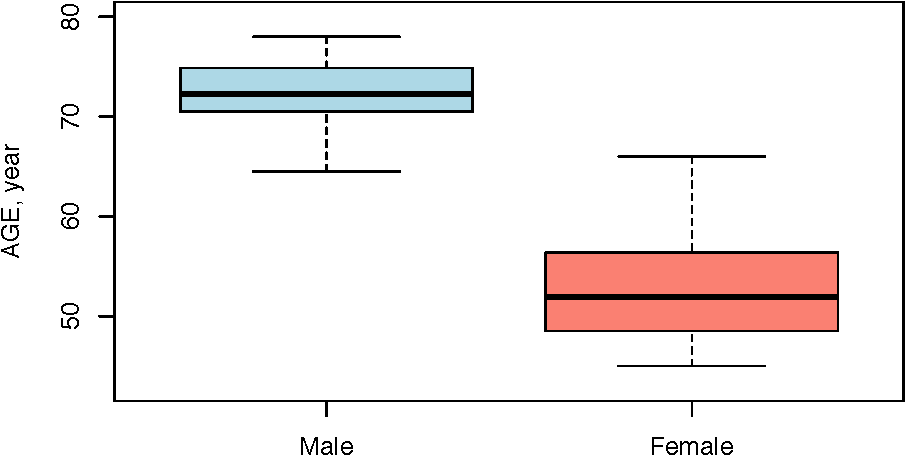
\includegraphics{Rprogramming_files/figure-latex/unnamed-chunk-7-1.pdf}

\subsection{Bar Plot}\label{bar-plot}

\begin{Shaded}
\begin{Highlighting}[]
\KeywordTok{barplot}\NormalTok{(d.demog}\OperatorTok{$}\NormalTok{HT)}
\end{Highlighting}
\end{Shaded}

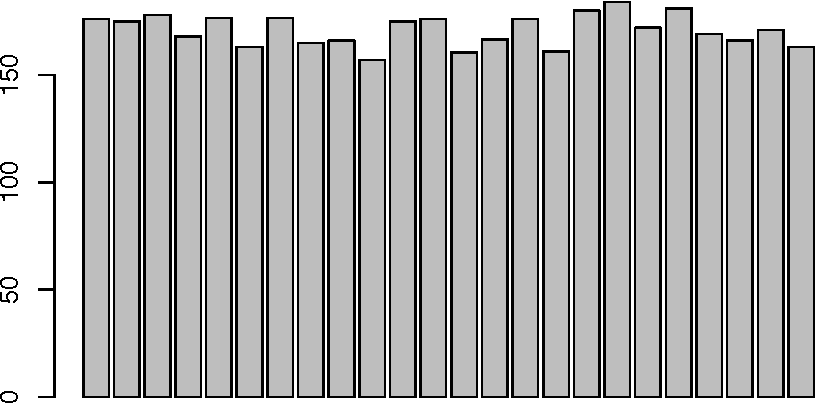
\includegraphics{Rprogramming_files/figure-latex/unnamed-chunk-8-1.pdf}

\begin{Shaded}
\begin{Highlighting}[]
\NormalTok{VADeaths}
\end{Highlighting}
\end{Shaded}

\begin{verbatim}
##       Rural Male Rural Female Urban Male Urban Female
## 50-54       11.7          8.7       15.4          8.4
## 55-59       18.1         11.7       24.3         13.6
## 60-64       26.9         20.3       37.0         19.3
## 65-69       41.0         30.9       54.6         35.1
## 70-74       66.0         54.3       71.1         50.0
\end{verbatim}

\begin{Shaded}
\begin{Highlighting}[]
\KeywordTok{barplot}\NormalTok{(VADeaths, }\DataTypeTok{border =} \StringTok{"dark blue"}\NormalTok{)}
\end{Highlighting}
\end{Shaded}

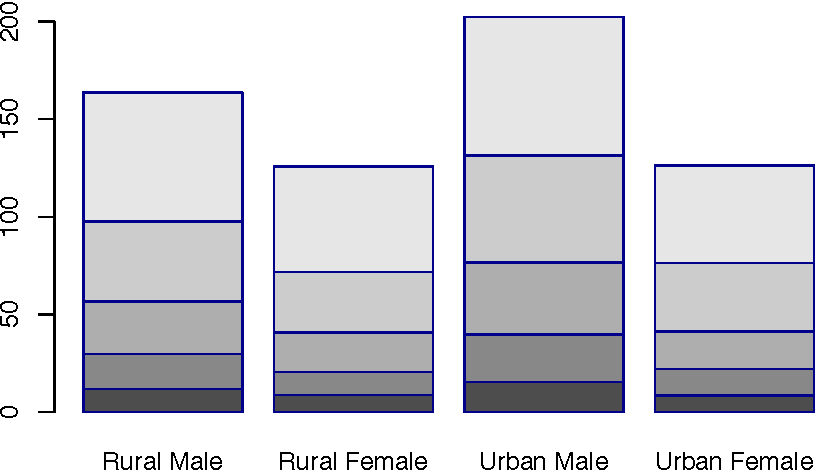
\includegraphics{Rprogramming_files/figure-latex/unnamed-chunk-8-2.pdf}

\begin{Shaded}
\begin{Highlighting}[]
\KeywordTok{barplot}\NormalTok{(VADeaths, }\DataTypeTok{col =} \KeywordTok{rainbow}\NormalTok{(}\DecValTok{20}\NormalTok{))}
\end{Highlighting}
\end{Shaded}

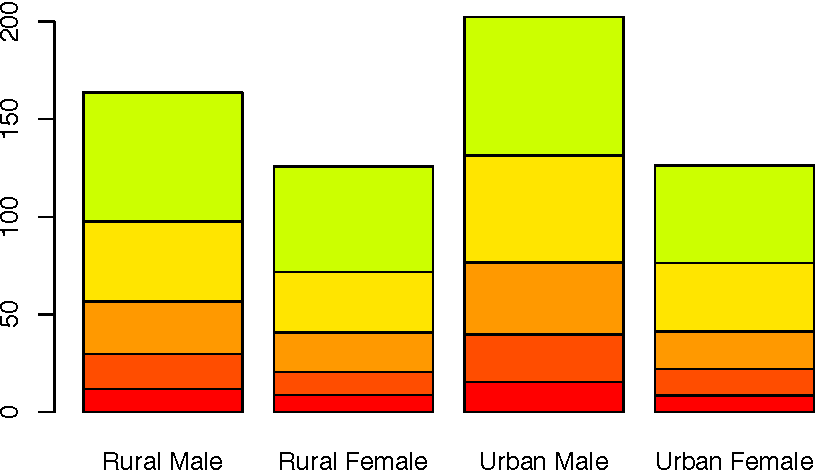
\includegraphics{Rprogramming_files/figure-latex/unnamed-chunk-8-3.pdf}

\begin{Shaded}
\begin{Highlighting}[]
\KeywordTok{barplot}\NormalTok{(VADeaths, }\DataTypeTok{col =} \KeywordTok{heat.colors}\NormalTok{(}\DecValTok{8}\NormalTok{))}
\end{Highlighting}
\end{Shaded}

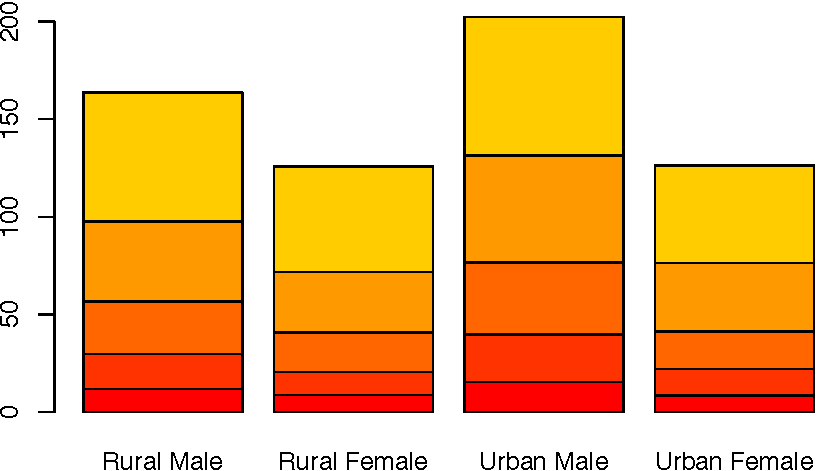
\includegraphics{Rprogramming_files/figure-latex/unnamed-chunk-8-4.pdf}

\begin{Shaded}
\begin{Highlighting}[]
\KeywordTok{barplot}\NormalTok{(VADeaths, }\DataTypeTok{col =} \KeywordTok{gray.colors}\NormalTok{(}\DecValTok{4}\NormalTok{))}
\end{Highlighting}
\end{Shaded}

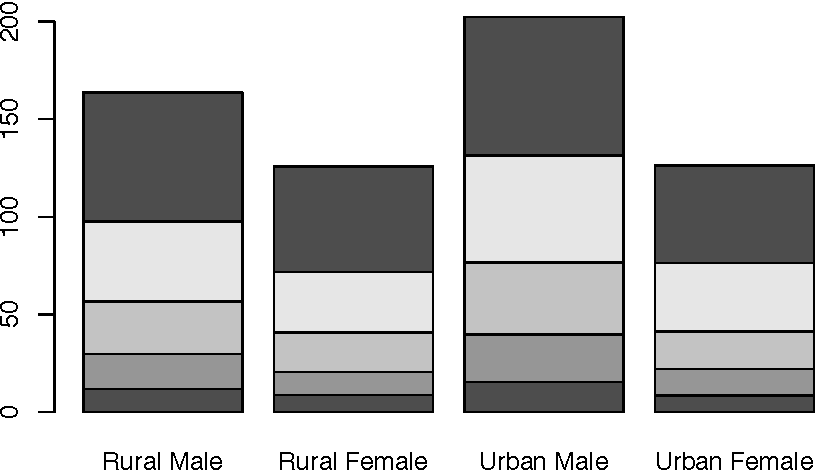
\includegraphics{Rprogramming_files/figure-latex/unnamed-chunk-8-5.pdf}

\begin{Shaded}
\begin{Highlighting}[]
\KeywordTok{barplot}\NormalTok{(VADeaths, }\DataTypeTok{col =} \KeywordTok{gray.colors}\NormalTok{(}\DecValTok{4}\NormalTok{), }\DataTypeTok{log=}\StringTok{"x"}\NormalTok{)}
\end{Highlighting}
\end{Shaded}

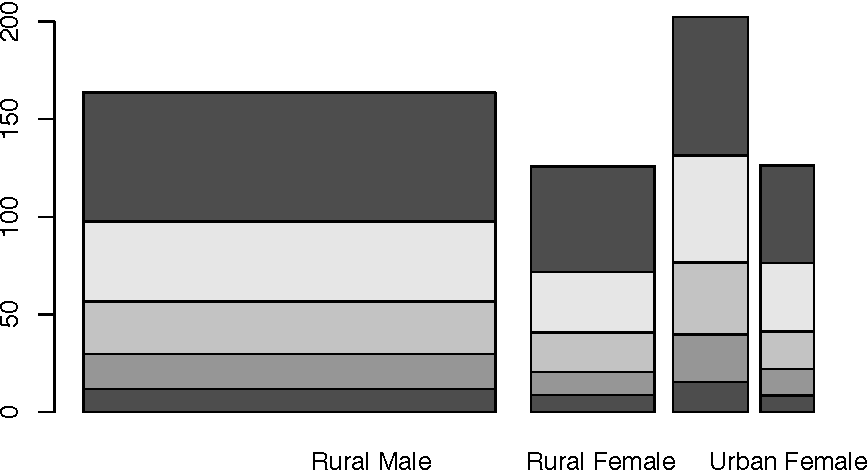
\includegraphics{Rprogramming_files/figure-latex/unnamed-chunk-8-6.pdf}

\begin{Shaded}
\begin{Highlighting}[]
\KeywordTok{barplot}\NormalTok{(VADeaths, }\DataTypeTok{col =} \KeywordTok{gray.colors}\NormalTok{(}\DecValTok{4}\NormalTok{), }\DataTypeTok{log=}\StringTok{"y"}\NormalTok{)}
\end{Highlighting}
\end{Shaded}

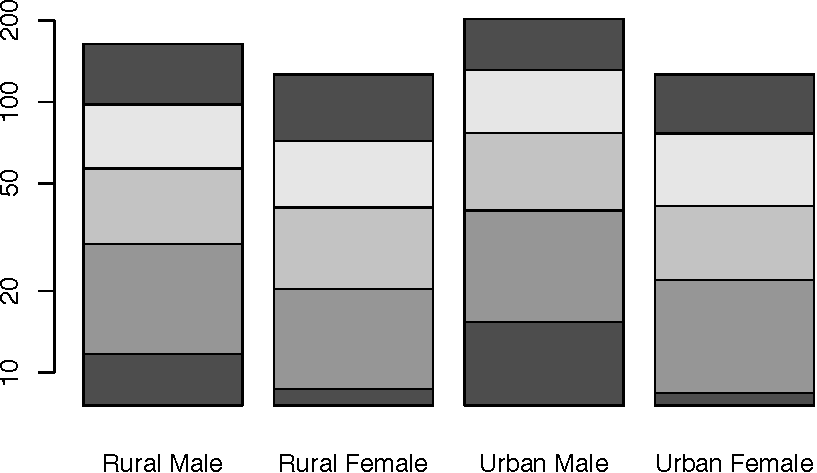
\includegraphics{Rprogramming_files/figure-latex/unnamed-chunk-8-7.pdf}

\begin{Shaded}
\begin{Highlighting}[]
\KeywordTok{barplot}\NormalTok{(VADeaths, }\DataTypeTok{col =} \KeywordTok{gray.colors}\NormalTok{(}\DecValTok{4}\NormalTok{), }\DataTypeTok{log=}\StringTok{"xy"}\NormalTok{)}
\end{Highlighting}
\end{Shaded}

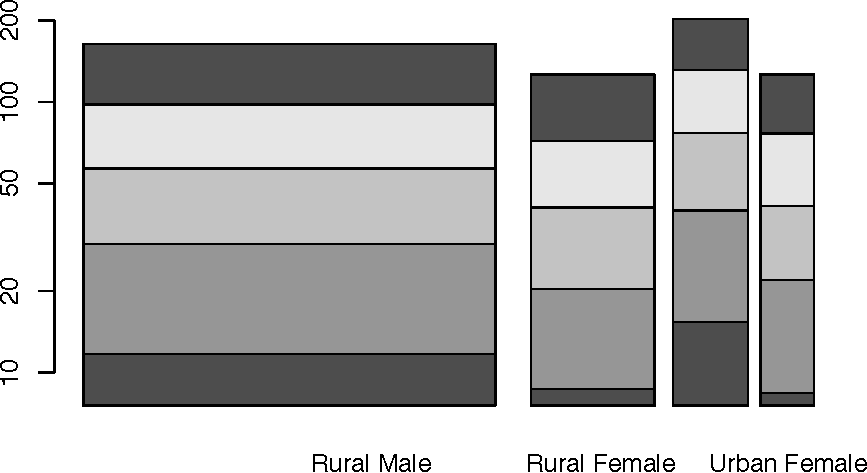
\includegraphics{Rprogramming_files/figure-latex/unnamed-chunk-8-8.pdf}

\subsection{pie chart}\label{pie-chart}

\begin{Shaded}
\begin{Highlighting}[]
\NormalTok{drug.X.market <-}\StringTok{ }\KeywordTok{c}\NormalTok{(}\FloatTok{0.12}\NormalTok{, }\FloatTok{0.29}\NormalTok{, }\FloatTok{0.32}\NormalTok{, }\FloatTok{0.22}\NormalTok{, }\FloatTok{0.11}\NormalTok{, }\FloatTok{0.28}\NormalTok{)}
\KeywordTok{names}\NormalTok{(drug.X.market) <-}\StringTok{ }\KeywordTok{c}\NormalTok{(}\StringTok{"South Korea"}\NormalTok{,}\StringTok{"China"}\NormalTok{,}\StringTok{"USA"}\NormalTok{,}\StringTok{"Japan"}\NormalTok{,}\StringTok{"Austria"}\NormalTok{,}\StringTok{"EU"}\NormalTok{)}
\KeywordTok{pie}\NormalTok{(drug.X.market)}
\end{Highlighting}
\end{Shaded}

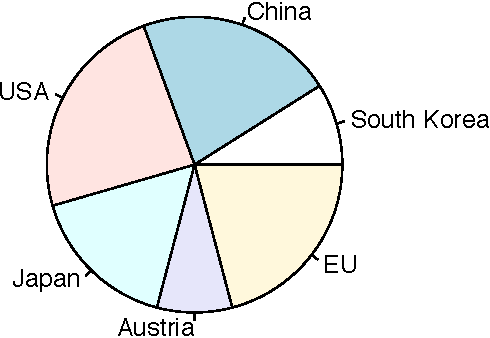
\includegraphics{Rprogramming_files/figure-latex/unnamed-chunk-9-1.pdf}

\subsection{matplot 함수}\label{matplot-}

\subsubsection{matrix와 column 사이의 그림}\label{matrix-column--}

\begin{Shaded}
\begin{Highlighting}[]
\NormalTok{pct.}\DecValTok{95}\NormalTok{ <-}\StringTok{ }\KeywordTok{read.csv}\NormalTok{(}\StringTok{"pct95.csv"}\NormalTok{)}
\KeywordTok{matplot}\NormalTok{(pct.}\DecValTok{95}\NormalTok{[,}\DecValTok{1}\NormalTok{], pct.}\DecValTok{95}\NormalTok{[,}\DecValTok{2}\OperatorTok{:}\KeywordTok{ncol}\NormalTok{(pct.}\DecValTok{95}\NormalTok{)], }\DataTypeTok{pch=}\DecValTok{1}\NormalTok{)}
\end{Highlighting}
\end{Shaded}

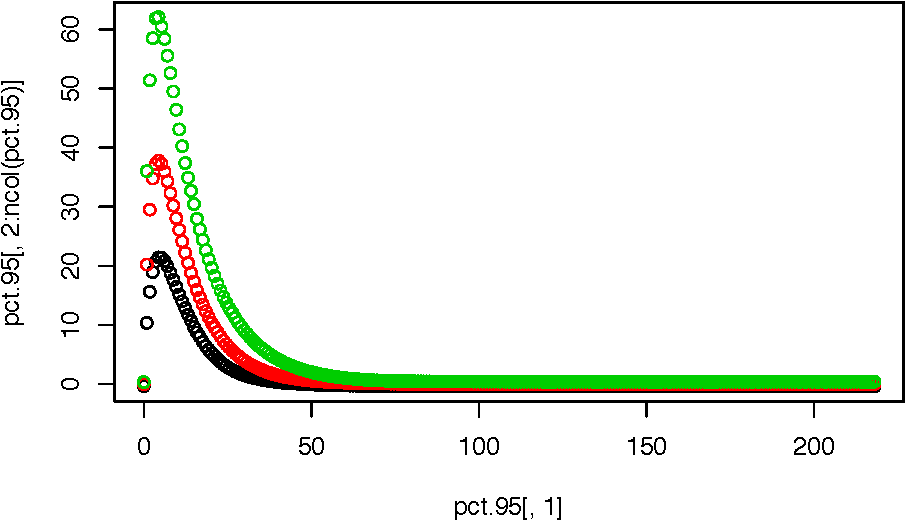
\includegraphics{Rprogramming_files/figure-latex/unnamed-chunk-10-1.pdf}

\begin{Shaded}
\begin{Highlighting}[]
\KeywordTok{matplot}\NormalTok{(pct.}\DecValTok{95}\NormalTok{[,}\DecValTok{1}\NormalTok{], pct.}\DecValTok{95}\NormalTok{[,}\DecValTok{2}\OperatorTok{:}\KeywordTok{ncol}\NormalTok{(pct.}\DecValTok{95}\NormalTok{)], }\DataTypeTok{pch=}\DecValTok{1}\NormalTok{, }\DataTypeTok{col=}\KeywordTok{c}\NormalTok{(}\DecValTok{1}\NormalTok{,}\DecValTok{2}\NormalTok{,}\DecValTok{1}\NormalTok{), }\DataTypeTok{type=}\StringTok{"l"}\NormalTok{, }\DataTypeTok{lty=}\DecValTok{1}\NormalTok{, }\DataTypeTok{lwd=}\KeywordTok{c}\NormalTok{(}\DecValTok{1}\NormalTok{,}\DecValTok{2}\NormalTok{,}\DecValTok{1}\NormalTok{))}
\end{Highlighting}
\end{Shaded}

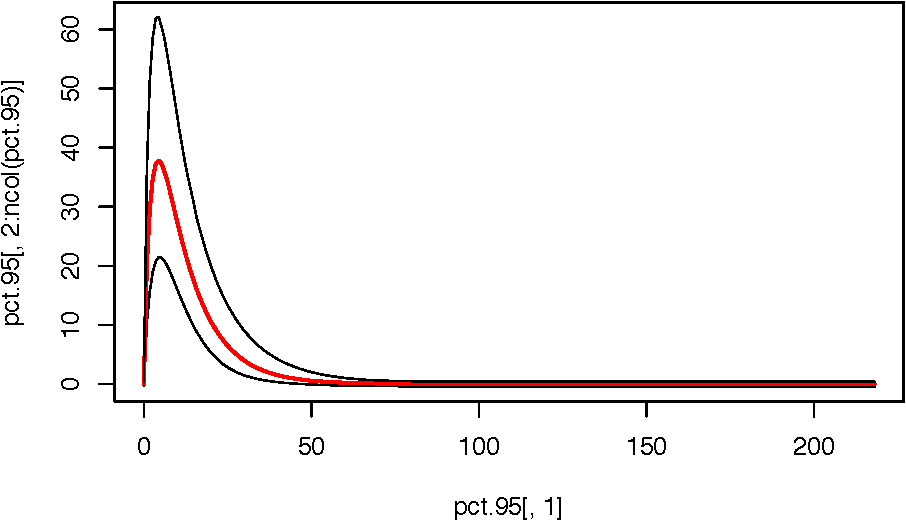
\includegraphics{Rprogramming_files/figure-latex/unnamed-chunk-10-2.pdf}

\subsection{Scatter plot matrices (pairs
plots)}\label{scatter-plot-matrices-pairs-plots}

\begin{Shaded}
\begin{Highlighting}[]
\KeywordTok{pairs}\NormalTok{(d.demog)}
\end{Highlighting}
\end{Shaded}

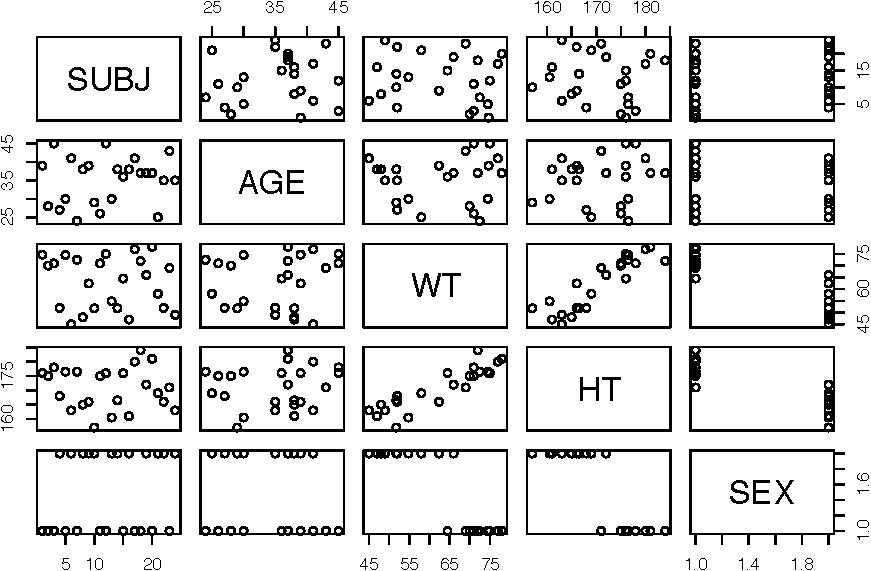
\includegraphics{Rprogramming_files/figure-latex/unnamed-chunk-11-1.pdf}

\subsubsection{add a loess smoother,
type}\label{add-a-loess-smoother-type}

\begin{Shaded}
\begin{Highlighting}[]
\KeywordTok{pairs}\NormalTok{(d.demog, }\DataTypeTok{panel =}\NormalTok{ panel.smooth)}
\end{Highlighting}
\end{Shaded}

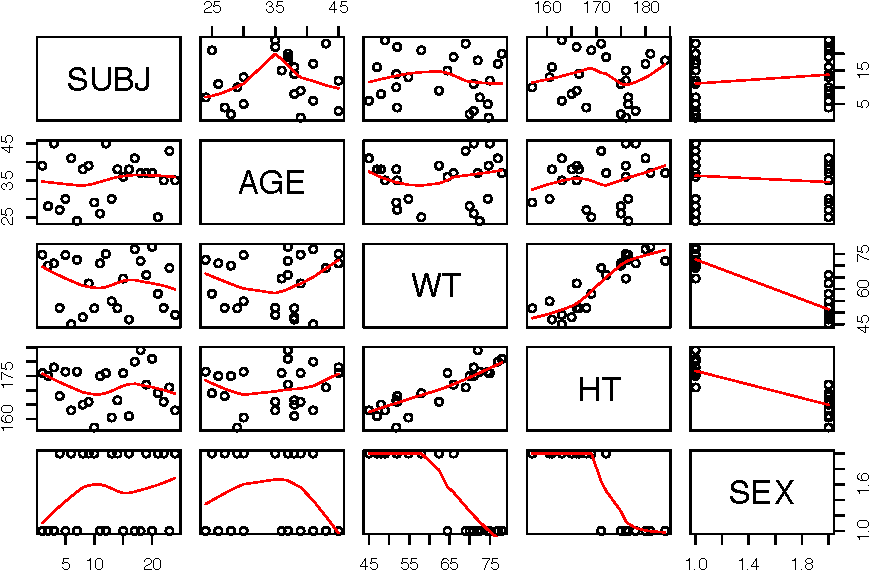
\includegraphics{Rprogramming_files/figure-latex/unnamed-chunk-12-1.pdf}

\begin{Shaded}
\begin{Highlighting}[]
\NormalTok{panel.cor <-}\StringTok{ }\ControlFlowTok{function}\NormalTok{(x, y, }\DataTypeTok{digits=}\DecValTok{2}\NormalTok{, }\DataTypeTok{prefix=}\StringTok{""}\NormalTok{, cex.cor)}
\NormalTok{\{}
\NormalTok{    usr <-}\StringTok{ }\KeywordTok{par}\NormalTok{(}\StringTok{"usr"}\NormalTok{); }\KeywordTok{on.exit}\NormalTok{(}\KeywordTok{par}\NormalTok{(usr))}
    \KeywordTok{par}\NormalTok{(}\DataTypeTok{usr =} \KeywordTok{c}\NormalTok{(}\DecValTok{0}\NormalTok{, }\DecValTok{1}\NormalTok{, }\DecValTok{0}\NormalTok{, }\DecValTok{1}\NormalTok{))}
\NormalTok{    r =}\StringTok{ }\NormalTok{(}\KeywordTok{cor}\NormalTok{(x, y))}
\NormalTok{    txt <-}\StringTok{ }\KeywordTok{format}\NormalTok{(}\KeywordTok{c}\NormalTok{(r, }\FloatTok{0.123456789}\NormalTok{), }\DataTypeTok{digits=}\NormalTok{digits)[}\DecValTok{1}\NormalTok{]}
\NormalTok{    txt <-}\StringTok{ }\KeywordTok{paste}\NormalTok{(prefix, txt, }\DataTypeTok{sep=}\StringTok{""}\NormalTok{)}
    \ControlFlowTok{if}\NormalTok{(}\KeywordTok{missing}\NormalTok{(cex.cor)) cex <-}\StringTok{ }\FloatTok{1.5}
    \KeywordTok{text}\NormalTok{(}\FloatTok{0.5}\NormalTok{, }\FloatTok{0.5}\NormalTok{, txt, }\DataTypeTok{cex =} \FloatTok{1.5}\NormalTok{)}
\NormalTok{\}}

\KeywordTok{pairs}\NormalTok{(d.demog, }\DataTypeTok{lower.panel=}\NormalTok{panel.smooth, }\DataTypeTok{upper.panel=}\NormalTok{panel.cor) }
\end{Highlighting}
\end{Shaded}

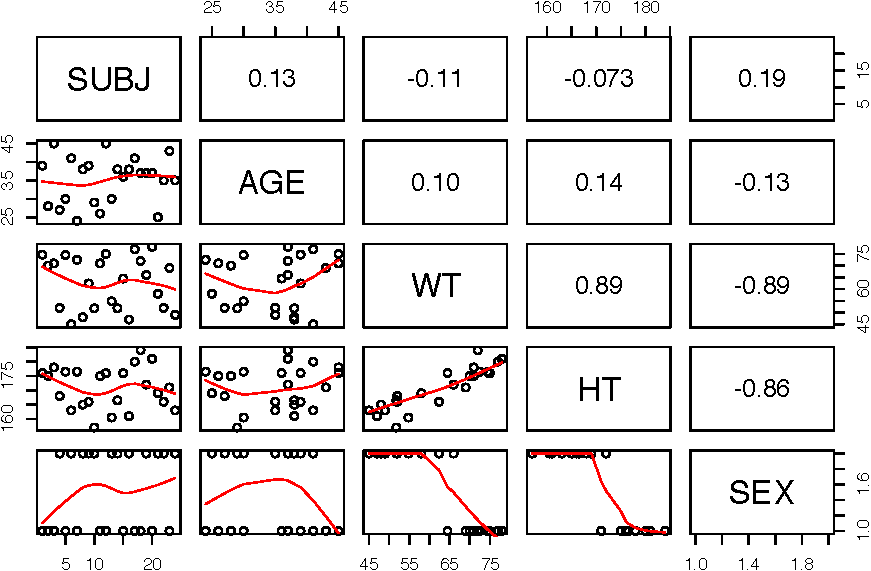
\includegraphics{Rprogramming_files/figure-latex/unnamed-chunk-12-2.pdf}

\section{하위수준 그림 함수}\label{lower}

\begin{itemize}
\tightlist
\item
  points : 점추가
\item
  lines : 선 추가
\item
  abline : 기준선 추가
\item
  mtext : 텍스트 추가
\item
  legend : 설명(legend) 추가
\item
  polygon : polygon 추가
\end{itemize}

\subsection{점, 선, 설명 추가 하기 \{add\}}\label{-----add}

\begin{Shaded}
\begin{Highlighting}[]
\KeywordTok{plot}\NormalTok{(pct.}\DecValTok{95}\OperatorTok{$}\NormalTok{TIME, pct.}\DecValTok{95}\OperatorTok{$}\NormalTok{PCT50, }\DataTypeTok{main=}\StringTok{"PK of Drug X"}
\NormalTok{     , }\DataTypeTok{type=}\StringTok{"l"}\NormalTok{, }\DataTypeTok{xlab=}\StringTok{"Time (h)"}\NormalTok{, }\DataTypeTok{ylab=}\StringTok{"Concentration (ng/ml)"}
\NormalTok{     , }\DataTypeTok{ylim=}\KeywordTok{range}\NormalTok{(}\DecValTok{0}\NormalTok{,}\DecValTok{80}\NormalTok{), }\DataTypeTok{lty=}\DecValTok{1}\NormalTok{, }\DataTypeTok{col=}\StringTok{"red"}\NormalTok{, }\DataTypeTok{lwd=}\DecValTok{2}\NormalTok{)}
\end{Highlighting}
\end{Shaded}

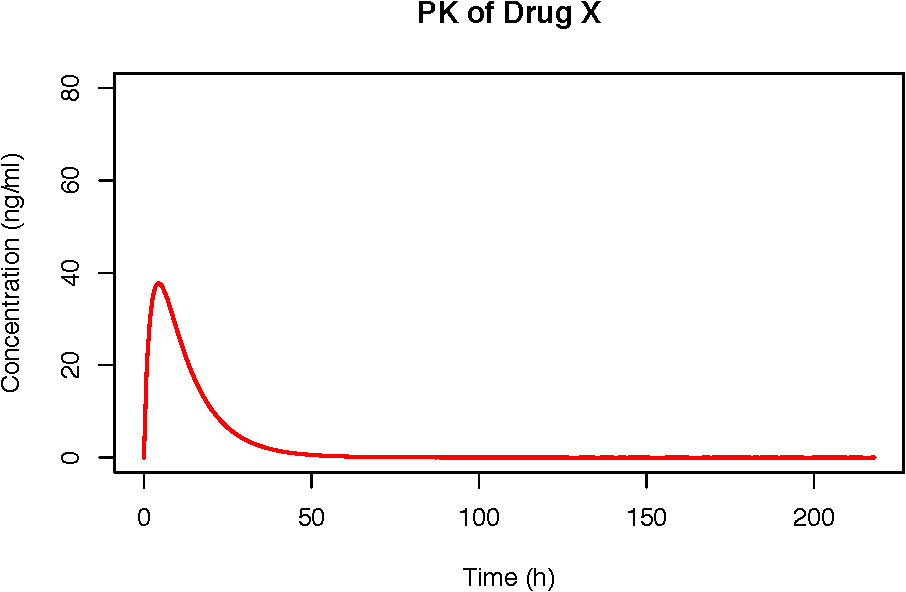
\includegraphics{Rprogramming_files/figure-latex/unnamed-chunk-13-1.pdf}

\begin{Shaded}
\begin{Highlighting}[]
\KeywordTok{plot}\NormalTok{(dta}\OperatorTok{$}\NormalTok{TIME[dta}\OperatorTok{$}\NormalTok{MDV}\OperatorTok{==}\DecValTok{0}\NormalTok{], dta}\OperatorTok{$}\NormalTok{DV[dta}\OperatorTok{$}\NormalTok{MDV}\OperatorTok{==}\DecValTok{0}\NormalTok{], }\DataTypeTok{main=}\StringTok{"PK of Drug X"}
\NormalTok{     , }\DataTypeTok{type=}\StringTok{"n"}\NormalTok{, }\DataTypeTok{xlab=}\StringTok{"Time (h)"}\NormalTok{, }\DataTypeTok{ylab=}\StringTok{"Concentration (ng/ml)"}
\NormalTok{     , }\DataTypeTok{ylim=}\KeywordTok{range}\NormalTok{(}\DecValTok{0}\NormalTok{,}\DecValTok{80}\NormalTok{))}
\KeywordTok{points}\NormalTok{(dta}\OperatorTok{$}\NormalTok{TIME[dta}\OperatorTok{$}\NormalTok{MDV}\OperatorTok{==}\DecValTok{0}\NormalTok{], dta}\OperatorTok{$}\NormalTok{DV[dta}\OperatorTok{$}\NormalTok{MDV}\OperatorTok{==}\DecValTok{0}\NormalTok{], }\DataTypeTok{pch =} \DecValTok{16}\NormalTok{, }\DataTypeTok{cex=}\FloatTok{0.8}\NormalTok{)}
\KeywordTok{lines}\NormalTok{(dta}\OperatorTok{$}\NormalTok{TIME[dta}\OperatorTok{$}\NormalTok{MDV}\OperatorTok{==}\DecValTok{0}\NormalTok{], dta}\OperatorTok{$}\NormalTok{DV[dta}\OperatorTok{$}\NormalTok{MDV}\OperatorTok{==}\DecValTok{0}\NormalTok{], }\DataTypeTok{col=}\StringTok{"black"}\NormalTok{, }\DataTypeTok{lwd=}\DecValTok{1}\NormalTok{)}
\KeywordTok{abline}\NormalTok{(}\DecValTok{40}\NormalTok{, }\DecValTok{0}\NormalTok{, }\DataTypeTok{col=}\StringTok{"red"}\NormalTok{, }\DataTypeTok{lty=}\DecValTok{2}\NormalTok{)                               }\CommentTok{# abline(a,b): y=a+b*x}
\KeywordTok{legend}\NormalTok{(}\StringTok{"topright"}\NormalTok{, }\DataTypeTok{legend=}\KeywordTok{c}\NormalTok{(}\StringTok{"Individual concentrations"}\NormalTok{)}
\NormalTok{       , }\DataTypeTok{lty=}\DecValTok{1}\NormalTok{, }\DataTypeTok{col=}\StringTok{"black"}\NormalTok{)}
\end{Highlighting}
\end{Shaded}

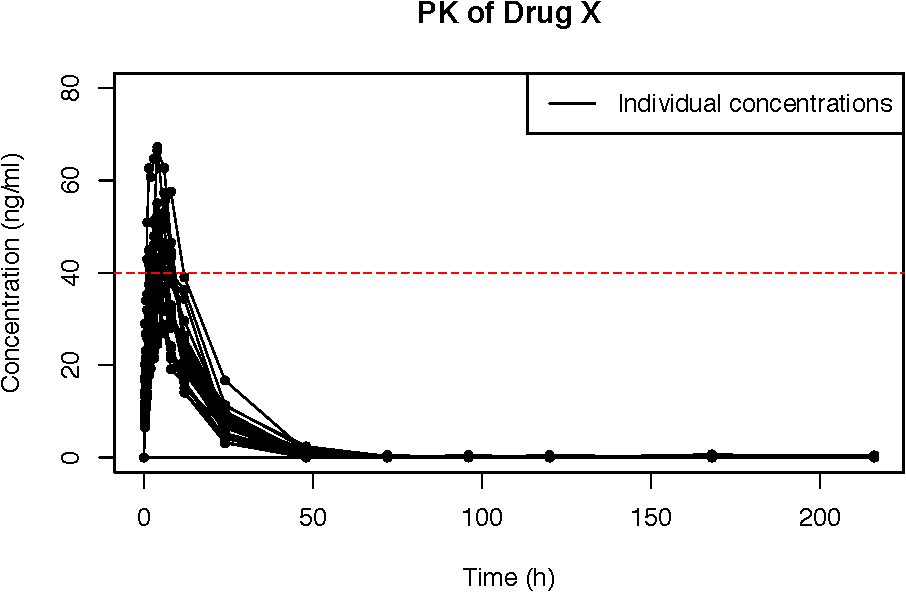
\includegraphics{Rprogramming_files/figure-latex/unnamed-chunk-13-2.pdf}

\subsection{polygon 함수}\label{polygon-}

\begin{Shaded}
\begin{Highlighting}[]
\KeywordTok{plot}\NormalTok{(}\KeywordTok{c}\NormalTok{(}\DecValTok{1}\NormalTok{, }\DecValTok{10}\NormalTok{), }\KeywordTok{c}\NormalTok{(}\DecValTok{1}\NormalTok{, }\DecValTok{6}\NormalTok{), }\DataTypeTok{type =} \StringTok{"n"}\NormalTok{)}
\KeywordTok{polygon}\NormalTok{(}\KeywordTok{c}\NormalTok{(}\DecValTok{2}\NormalTok{,}\DecValTok{8}\NormalTok{,}\DecValTok{8}\NormalTok{,}\DecValTok{2}\NormalTok{), }\KeywordTok{c}\NormalTok{(}\DecValTok{5}\NormalTok{,}\DecValTok{4}\NormalTok{,}\DecValTok{3}\NormalTok{,}\DecValTok{2}\NormalTok{), }\DataTypeTok{col=}\StringTok{"lightgreen"}\NormalTok{)}
\end{Highlighting}
\end{Shaded}

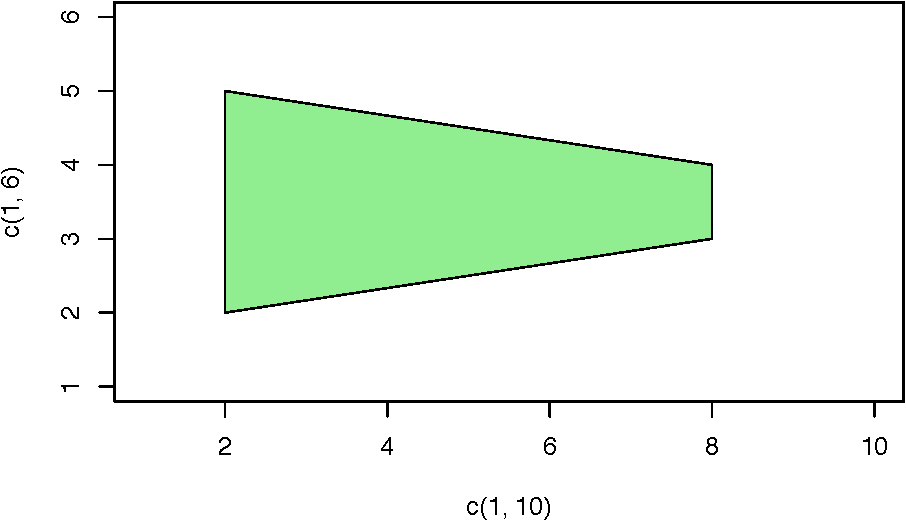
\includegraphics{Rprogramming_files/figure-latex/unnamed-chunk-14-1.pdf}

\begin{Shaded}
\begin{Highlighting}[]
\KeywordTok{plot}\NormalTok{(}\KeywordTok{c}\NormalTok{(}\DecValTok{1}\NormalTok{, }\DecValTok{9}\NormalTok{), }\DecValTok{1}\OperatorTok{:}\DecValTok{2}\NormalTok{, }\DataTypeTok{type =} \StringTok{"n"}\NormalTok{)}
\KeywordTok{polygon}\NormalTok{(}\DecValTok{1}\OperatorTok{:}\DecValTok{9}\NormalTok{, }\KeywordTok{c}\NormalTok{(}\DecValTok{2}\NormalTok{,}\DecValTok{1}\NormalTok{,}\DecValTok{2}\NormalTok{,}\DecValTok{1}\NormalTok{,}\DecValTok{1}\NormalTok{,}\DecValTok{2}\NormalTok{,}\DecValTok{1}\NormalTok{,}\DecValTok{2}\NormalTok{,}\DecValTok{1}\NormalTok{),}
        \DataTypeTok{col =} \KeywordTok{c}\NormalTok{(}\StringTok{"red"}\NormalTok{, }\StringTok{"blue"}\NormalTok{),}
        \DataTypeTok{border =} \KeywordTok{c}\NormalTok{(}\StringTok{"green"}\NormalTok{, }\StringTok{"yellow"}\NormalTok{),}
        \DataTypeTok{lwd =} \DecValTok{3}\NormalTok{, }\DataTypeTok{lty =} \KeywordTok{c}\NormalTok{(}\StringTok{"dashed"}\NormalTok{, }\StringTok{"solid"}\NormalTok{))}
\end{Highlighting}
\end{Shaded}

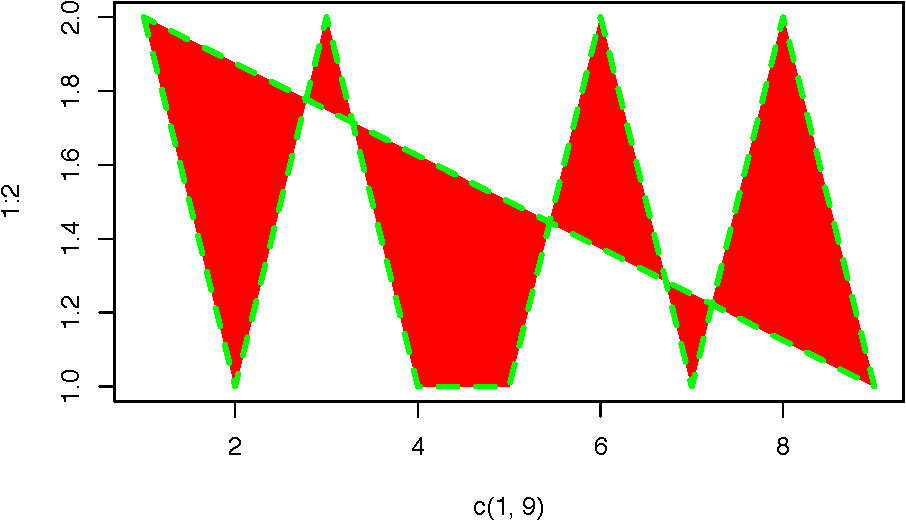
\includegraphics{Rprogramming_files/figure-latex/unnamed-chunk-14-2.pdf}

\section{그림 출력하기}\label{print}

\subsection{pdf graphics devices}\label{pdf-graphics-devices}

\begin{Shaded}
\begin{Highlighting}[]
\KeywordTok{pdf}\NormalTok{(}\StringTok{"PK_of_Drug_X.pdf"}\NormalTok{)}

\KeywordTok{plot}\NormalTok{(dta}\OperatorTok{$}\NormalTok{TIME[dta}\OperatorTok{$}\NormalTok{MDV}\OperatorTok{==}\DecValTok{0}\NormalTok{], dta}\OperatorTok{$}\NormalTok{DV[dta}\OperatorTok{$}\NormalTok{MDV}\OperatorTok{==}\DecValTok{0}\NormalTok{], }\DataTypeTok{main=}\StringTok{"PK of Drug X"}
\NormalTok{     , }\DataTypeTok{type=}\StringTok{"n"}\NormalTok{, }\DataTypeTok{xlab=}\StringTok{"Time (h)"}\NormalTok{, }\DataTypeTok{ylab=}\StringTok{"Concentration (ng/ml)"}
\NormalTok{     , }\DataTypeTok{ylim=}\KeywordTok{range}\NormalTok{(}\DecValTok{0}\NormalTok{,}\DecValTok{80}\NormalTok{))}
\KeywordTok{points}\NormalTok{(dta}\OperatorTok{$}\NormalTok{TIME[dta}\OperatorTok{$}\NormalTok{MDV}\OperatorTok{==}\DecValTok{0}\NormalTok{], dta}\OperatorTok{$}\NormalTok{DV[dta}\OperatorTok{$}\NormalTok{MDV}\OperatorTok{==}\DecValTok{0}\NormalTok{], }\DataTypeTok{pch =} \DecValTok{16}\NormalTok{, }\DataTypeTok{cex=}\FloatTok{0.8}\NormalTok{)}
\KeywordTok{lines}\NormalTok{(dta}\OperatorTok{$}\NormalTok{TIME[dta}\OperatorTok{$}\NormalTok{MDV}\OperatorTok{==}\DecValTok{0}\NormalTok{], dta}\OperatorTok{$}\NormalTok{DV[dta}\OperatorTok{$}\NormalTok{MDV}\OperatorTok{==}\DecValTok{0}\NormalTok{], }\DataTypeTok{col=}\StringTok{"black"}\NormalTok{, }\DataTypeTok{lwd=}\DecValTok{1}\NormalTok{)}
\KeywordTok{abline}\NormalTok{(}\DecValTok{40}\NormalTok{, }\DecValTok{0}\NormalTok{, }\DataTypeTok{col=}\StringTok{"red"}\NormalTok{, }\DataTypeTok{lty=}\DecValTok{2}\NormalTok{)                               }\CommentTok{#abline(a,b): y=a+b*x}
\KeywordTok{legend}\NormalTok{(}\StringTok{"topright"}\NormalTok{, }\DataTypeTok{legend=}\KeywordTok{c}\NormalTok{(}\StringTok{"Individual concentrations"}\NormalTok{)}
\NormalTok{       , }\DataTypeTok{lty=}\DecValTok{1}\NormalTok{, }\DataTypeTok{col=}\StringTok{"black"}\NormalTok{)}

\KeywordTok{dev.off}\NormalTok{()}
\end{Highlighting}
\end{Shaded}

\begin{verbatim}
## pdf 
##   2
\end{verbatim}

\subsection{PNG graphics devices}\label{png-graphics-devices}

\begin{Shaded}
\begin{Highlighting}[]
\KeywordTok{png}\NormalTok{(}\StringTok{"PK_of_Drug_X.png"}\NormalTok{)}

\KeywordTok{plot}\NormalTok{(dta}\OperatorTok{$}\NormalTok{TIME[dta}\OperatorTok{$}\NormalTok{MDV}\OperatorTok{==}\DecValTok{0}\NormalTok{], dta}\OperatorTok{$}\NormalTok{DV[dta}\OperatorTok{$}\NormalTok{MDV}\OperatorTok{==}\DecValTok{0}\NormalTok{], }\DataTypeTok{main=}\StringTok{"PK of Drug X"}
\NormalTok{     , }\DataTypeTok{type=}\StringTok{"n"}\NormalTok{, }\DataTypeTok{xlab=}\StringTok{"Time (h)"}\NormalTok{, }\DataTypeTok{ylab=}\StringTok{"Concentration (ng/ml)"}
\NormalTok{     , }\DataTypeTok{ylim=}\KeywordTok{range}\NormalTok{(}\DecValTok{0}\NormalTok{,}\DecValTok{80}\NormalTok{))}
\KeywordTok{points}\NormalTok{(dta}\OperatorTok{$}\NormalTok{TIME[dta}\OperatorTok{$}\NormalTok{MDV}\OperatorTok{==}\DecValTok{0}\NormalTok{], dta}\OperatorTok{$}\NormalTok{DV[dta}\OperatorTok{$}\NormalTok{MDV}\OperatorTok{==}\DecValTok{0}\NormalTok{], }\DataTypeTok{pch =} \DecValTok{16}\NormalTok{, }\DataTypeTok{cex=}\FloatTok{0.8}\NormalTok{)}
\KeywordTok{lines}\NormalTok{(dta}\OperatorTok{$}\NormalTok{TIME[dta}\OperatorTok{$}\NormalTok{MDV}\OperatorTok{==}\DecValTok{0}\NormalTok{], dta}\OperatorTok{$}\NormalTok{DV[dta}\OperatorTok{$}\NormalTok{MDV}\OperatorTok{==}\DecValTok{0}\NormalTok{], }\DataTypeTok{col=}\StringTok{"black"}\NormalTok{, }\DataTypeTok{lwd=}\DecValTok{1}\NormalTok{)}
\KeywordTok{abline}\NormalTok{(}\DecValTok{40}\NormalTok{, }\DecValTok{0}\NormalTok{, }\DataTypeTok{col=}\StringTok{"red"}\NormalTok{, }\DataTypeTok{lty=}\DecValTok{2}\NormalTok{)                               }\CommentTok{#abline(a,b): y=a+b*x}
\KeywordTok{legend}\NormalTok{(}\StringTok{"topright"}\NormalTok{, }\DataTypeTok{legend=}\KeywordTok{c}\NormalTok{(}\StringTok{"Individual concentrations"}\NormalTok{)}
\NormalTok{       , }\DataTypeTok{lty=}\DecValTok{1}\NormalTok{, }\DataTypeTok{col=}\StringTok{"black"}\NormalTok{)}

\KeywordTok{dev.off}\NormalTok{()}
\end{Highlighting}
\end{Shaded}

\begin{verbatim}
## pdf 
##   2
\end{verbatim}

\chapter{Data Import / Export}\label{data-import-export}

\begin{quote}
2017-03-29 배균섭 교수님 강의
\end{quote}

이번 시간에는 자료를 불러오고 조작을 가한 뒤 저장하는 방법에 대해
알아보겠습니다.

\section{Read.csv}\label{read.csv}

\begin{Shaded}
\begin{Highlighting}[]
\KeywordTok{setwd}\NormalTok{(}\StringTok{"D:/Rt"}\NormalTok{)}
\KeywordTok{dir}\NormalTok{()}
\NormalTok{mydata =}\StringTok{ }\KeywordTok{read.csv}\NormalTok{(}\StringTok{"MyData2017.csv"}\NormalTok{, }\DataTypeTok{as.is=}\OtherTok{TRUE}\NormalTok{)}
\end{Highlighting}
\end{Shaded}

\section{Theoph 데이타}\label{theoph-}

R에 기본적으로 들어있는 약동학 자료에 대해 살펴보겠습니다.

\begin{Shaded}
\begin{Highlighting}[]
\NormalTok{Theoph}
\end{Highlighting}
\end{Shaded}

\begin{verbatim}
##     Subject   Wt Dose  Time  conc
## 1         1 79.6 4.02  0.00  0.74
## 2         1 79.6 4.02  0.25  2.84
## 3         1 79.6 4.02  0.57  6.57
## 4         1 79.6 4.02  1.12 10.50
## 5         1 79.6 4.02  2.02  9.66
## 6         1 79.6 4.02  3.82  8.58
## 7         1 79.6 4.02  5.10  8.36
## 8         1 79.6 4.02  7.03  7.47
## 9         1 79.6 4.02  9.05  6.89
## 10        1 79.6 4.02 12.12  5.94
## 11        1 79.6 4.02 24.37  3.28
## 12        2 72.4 4.40  0.00  0.00
## 13        2 72.4 4.40  0.27  1.72
## 14        2 72.4 4.40  0.52  7.91
## 15        2 72.4 4.40  1.00  8.31
## 16        2 72.4 4.40  1.92  8.33
## 17        2 72.4 4.40  3.50  6.85
## 18        2 72.4 4.40  5.02  6.08
## 19        2 72.4 4.40  7.03  5.40
## 20        2 72.4 4.40  9.00  4.55
## 21        2 72.4 4.40 12.00  3.01
## 22        2 72.4 4.40 24.30  0.90
## 23        3 70.5 4.53  0.00  0.00
## 24        3 70.5 4.53  0.27  4.40
## 25        3 70.5 4.53  0.58  6.90
## 26        3 70.5 4.53  1.02  8.20
## 27        3 70.5 4.53  2.02  7.80
## 28        3 70.5 4.53  3.62  7.50
## 29        3 70.5 4.53  5.08  6.20
## 30        3 70.5 4.53  7.07  5.30
## 31        3 70.5 4.53  9.00  4.90
## 32        3 70.5 4.53 12.15  3.70
## 33        3 70.5 4.53 24.17  1.05
## 34        4 72.7 4.40  0.00  0.00
## 35        4 72.7 4.40  0.35  1.89
## 36        4 72.7 4.40  0.60  4.60
## 37        4 72.7 4.40  1.07  8.60
## 38        4 72.7 4.40  2.13  8.38
## 39        4 72.7 4.40  3.50  7.54
## 40        4 72.7 4.40  5.02  6.88
## 41        4 72.7 4.40  7.02  5.78
## 42        4 72.7 4.40  9.02  5.33
## 43        4 72.7 4.40 11.98  4.19
## 44        4 72.7 4.40 24.65  1.15
## 45        5 54.6 5.86  0.00  0.00
## 46        5 54.6 5.86  0.30  2.02
## 47        5 54.6 5.86  0.52  5.63
## 48        5 54.6 5.86  1.00 11.40
## 49        5 54.6 5.86  2.02  9.33
## 50        5 54.6 5.86  3.50  8.74
## 51        5 54.6 5.86  5.02  7.56
## 52        5 54.6 5.86  7.02  7.09
## 53        5 54.6 5.86  9.10  5.90
## 54        5 54.6 5.86 12.00  4.37
## 55        5 54.6 5.86 24.35  1.57
## 56        6 80.0 4.00  0.00  0.00
## 57        6 80.0 4.00  0.27  1.29
## 58        6 80.0 4.00  0.58  3.08
## 59        6 80.0 4.00  1.15  6.44
## 60        6 80.0 4.00  2.03  6.32
## 61        6 80.0 4.00  3.57  5.53
## 62        6 80.0 4.00  5.00  4.94
## 63        6 80.0 4.00  7.00  4.02
## 64        6 80.0 4.00  9.22  3.46
## 65        6 80.0 4.00 12.10  2.78
## 66        6 80.0 4.00 23.85  0.92
## 67        7 64.6 4.95  0.00  0.15
## 68        7 64.6 4.95  0.25  0.85
## 69        7 64.6 4.95  0.50  2.35
## 70        7 64.6 4.95  1.02  5.02
## 71        7 64.6 4.95  2.02  6.58
## 72        7 64.6 4.95  3.48  7.09
## 73        7 64.6 4.95  5.00  6.66
## 74        7 64.6 4.95  6.98  5.25
## 75        7 64.6 4.95  9.00  4.39
## 76        7 64.6 4.95 12.05  3.53
## 77        7 64.6 4.95 24.22  1.15
## 78        8 70.5 4.53  0.00  0.00
## 79        8 70.5 4.53  0.25  3.05
## 80        8 70.5 4.53  0.52  3.05
## 81        8 70.5 4.53  0.98  7.31
## 82        8 70.5 4.53  2.02  7.56
## 83        8 70.5 4.53  3.53  6.59
## 84        8 70.5 4.53  5.05  5.88
## 85        8 70.5 4.53  7.15  4.73
## 86        8 70.5 4.53  9.07  4.57
## 87        8 70.5 4.53 12.10  3.00
## 88        8 70.5 4.53 24.12  1.25
## 89        9 86.4 3.10  0.00  0.00
## 90        9 86.4 3.10  0.30  7.37
## 91        9 86.4 3.10  0.63  9.03
## 92        9 86.4 3.10  1.05  7.14
## 93        9 86.4 3.10  2.02  6.33
## 94        9 86.4 3.10  3.53  5.66
## 95        9 86.4 3.10  5.02  5.67
## 96        9 86.4 3.10  7.17  4.24
## 97        9 86.4 3.10  8.80  4.11
## 98        9 86.4 3.10 11.60  3.16
## 99        9 86.4 3.10 24.43  1.12
## 100      10 58.2 5.50  0.00  0.24
## 101      10 58.2 5.50  0.37  2.89
## 102      10 58.2 5.50  0.77  5.22
## 103      10 58.2 5.50  1.02  6.41
## 104      10 58.2 5.50  2.05  7.83
## 105      10 58.2 5.50  3.55 10.21
## 106      10 58.2 5.50  5.05  9.18
## 107      10 58.2 5.50  7.08  8.02
## 108      10 58.2 5.50  9.38  7.14
## 109      10 58.2 5.50 12.10  5.68
## 110      10 58.2 5.50 23.70  2.42
## 111      11 65.0 4.92  0.00  0.00
## 112      11 65.0 4.92  0.25  4.86
## 113      11 65.0 4.92  0.50  7.24
## 114      11 65.0 4.92  0.98  8.00
## 115      11 65.0 4.92  1.98  6.81
## 116      11 65.0 4.92  3.60  5.87
## 117      11 65.0 4.92  5.02  5.22
## 118      11 65.0 4.92  7.03  4.45
## 119      11 65.0 4.92  9.03  3.62
## 120      11 65.0 4.92 12.12  2.69
## 121      11 65.0 4.92 24.08  0.86
## 122      12 60.5 5.30  0.00  0.00
## 123      12 60.5 5.30  0.25  1.25
## 124      12 60.5 5.30  0.50  3.96
## 125      12 60.5 5.30  1.00  7.82
## 126      12 60.5 5.30  2.00  9.72
## 127      12 60.5 5.30  3.52  9.75
## 128      12 60.5 5.30  5.07  8.57
## 129      12 60.5 5.30  7.07  6.59
## 130      12 60.5 5.30  9.03  6.11
## 131      12 60.5 5.30 12.05  4.57
## 132      12 60.5 5.30 24.15  1.17
\end{verbatim}

R console에서 \texttt{?Theoph}를 타이핑 치면 좀 더 자세한 정보를 얻을 수
있습니다.

\section{lattice}\label{lattice}

lattice 패키지를 불러온 뒤 그림을 그려보겠습니다. \citep{R-lattice}

\begin{Shaded}
\begin{Highlighting}[]
\KeywordTok{library}\NormalTok{(lattice) }\CommentTok{# trellis}

\KeywordTok{xyplot}\NormalTok{(conc }\OperatorTok{~}\StringTok{ }\NormalTok{Time }\OperatorTok{|}\StringTok{ }\NormalTok{Subject, }\DataTypeTok{data=}\NormalTok{Theoph)}
\end{Highlighting}
\end{Shaded}

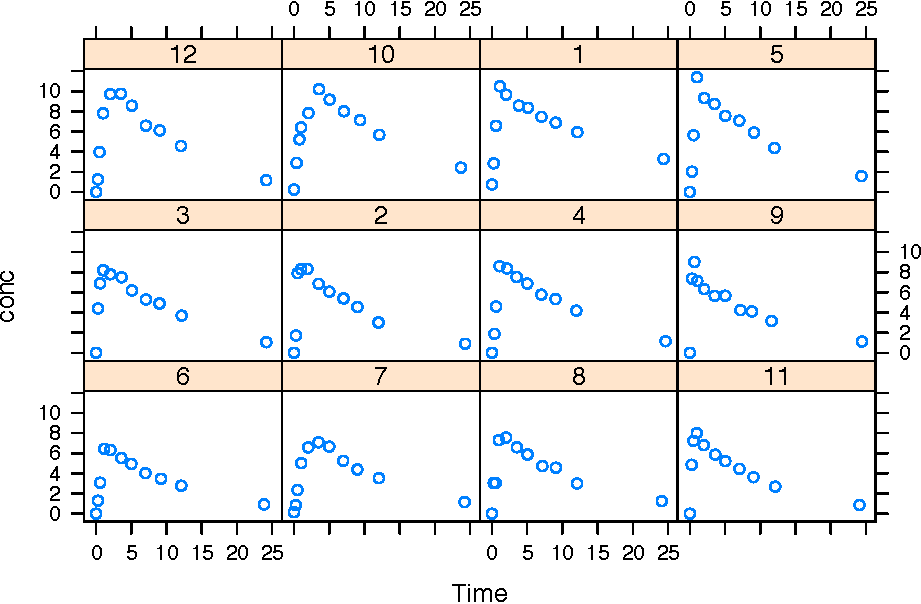
\includegraphics{Rprogramming_files/figure-latex/unnamed-chunk-19-1.pdf}

\begin{Shaded}
\begin{Highlighting}[]
\KeywordTok{xyplot}\NormalTok{(conc }\OperatorTok{~}\StringTok{ }\NormalTok{Time }\OperatorTok{|}\StringTok{ }\NormalTok{Subject, }\DataTypeTok{data=}\NormalTok{Theoph, }\DataTypeTok{type=}\StringTok{"b"}\NormalTok{)}
\end{Highlighting}
\end{Shaded}

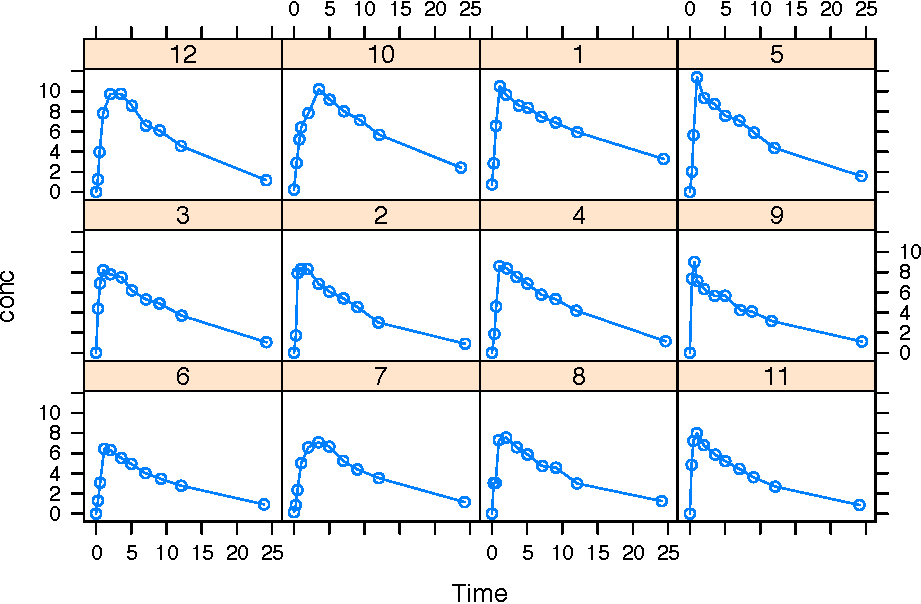
\includegraphics{Rprogramming_files/figure-latex/unnamed-chunk-19-2.pdf}

\begin{Shaded}
\begin{Highlighting}[]
\NormalTok{Theoph[,}\StringTok{"ID"}\NormalTok{] =}\StringTok{ }\KeywordTok{as.numeric}\NormalTok{(}\KeywordTok{as.character}\NormalTok{(Theoph[,}\StringTok{"Subject"}\NormalTok{]))}

\KeywordTok{xyplot}\NormalTok{(conc }\OperatorTok{~}\StringTok{ }\NormalTok{Time }\OperatorTok{|}\StringTok{ }\NormalTok{ID, }\DataTypeTok{data=}\NormalTok{Theoph, }\DataTypeTok{type=}\StringTok{"b"}\NormalTok{)}
\end{Highlighting}
\end{Shaded}

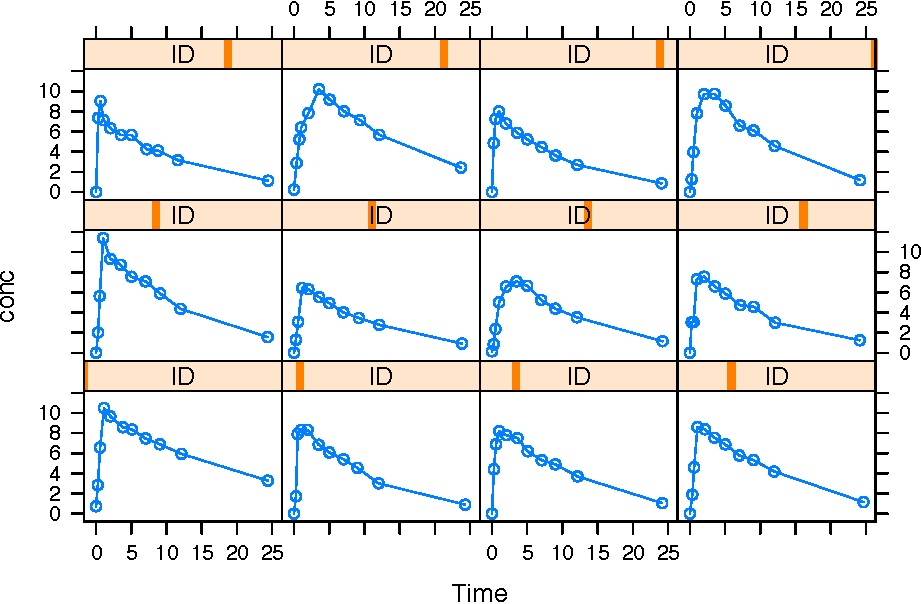
\includegraphics{Rprogramming_files/figure-latex/unnamed-chunk-19-3.pdf}

\begin{Shaded}
\begin{Highlighting}[]
\KeywordTok{xyplot}\NormalTok{(conc }\OperatorTok{~}\StringTok{ }\NormalTok{Time }\OperatorTok{|}\StringTok{ }\KeywordTok{as.factor}\NormalTok{(ID), }\DataTypeTok{data=}\NormalTok{Theoph, }\DataTypeTok{type=}\StringTok{"b"}\NormalTok{)}
\end{Highlighting}
\end{Shaded}

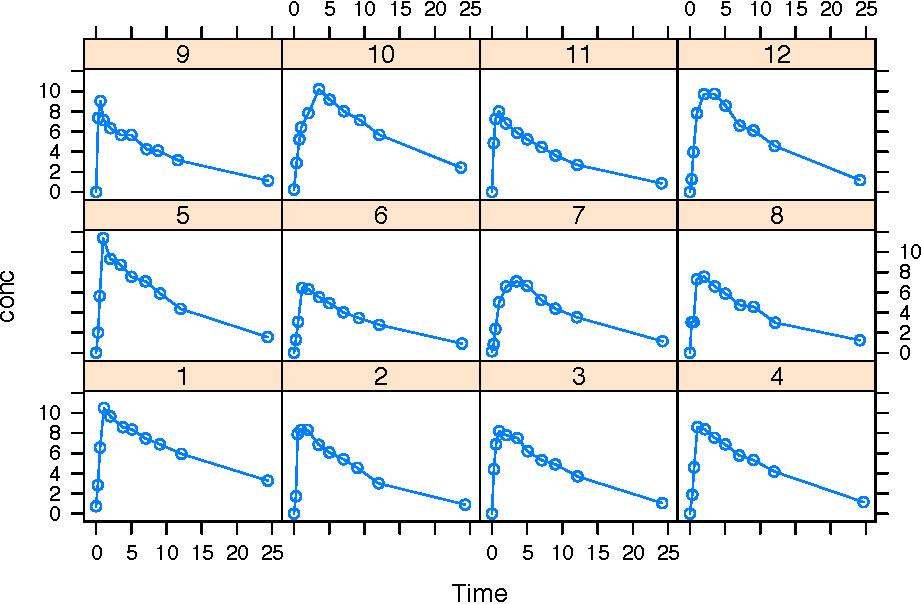
\includegraphics{Rprogramming_files/figure-latex/unnamed-chunk-19-4.pdf}

\begin{Shaded}
\begin{Highlighting}[]
\KeywordTok{write.csv}\NormalTok{(Theoph, }\StringTok{"Theoph.csv"}\NormalTok{, }\DataTypeTok{row.names=}\OtherTok{FALSE}\NormalTok{, }\DataTypeTok{quote=}\OtherTok{FALSE}\NormalTok{, }\DataTypeTok{na=}\StringTok{""}\NormalTok{)}
\end{Highlighting}
\end{Shaded}

\section{Subseting and write.csv}\label{subseting-and-write.csv}

자료를 편집하고, subset을 만들고 각각을 파일로 저장하는 방법에 대해
알아보겠습니다.

\begin{Shaded}
\begin{Highlighting}[]
\NormalTok{IDs =}\StringTok{ }\KeywordTok{sort}\NormalTok{(}\KeywordTok{unique}\NormalTok{(Theoph[,}\StringTok{"ID"}\NormalTok{])) ; IDs}
\end{Highlighting}
\end{Shaded}

\begin{verbatim}
##  [1]  1  2  3  4  5  6  7  8  9 10 11 12
\end{verbatim}

\begin{Shaded}
\begin{Highlighting}[]
\NormalTok{nID =}\StringTok{ }\KeywordTok{length}\NormalTok{(IDs) ; nID}
\end{Highlighting}
\end{Shaded}

\begin{verbatim}
## [1] 12
\end{verbatim}

\begin{Shaded}
\begin{Highlighting}[]
\NormalTok{demog =}\StringTok{ }\KeywordTok{unique}\NormalTok{(Theoph[,}\KeywordTok{c}\NormalTok{(}\StringTok{"ID"}\NormalTok{,}\StringTok{"Wt"}\NormalTok{)])}
\KeywordTok{colnames}\NormalTok{(demog) =}\StringTok{ }\KeywordTok{c}\NormalTok{(}\StringTok{"ID"}\NormalTok{, }\StringTok{"BWT"}\NormalTok{)}
\KeywordTok{write.csv}\NormalTok{(demog, }\StringTok{"1-demog.csv"}\NormalTok{, }\DataTypeTok{row.names=}\OtherTok{FALSE}\NormalTok{, }\DataTypeTok{quote=}\OtherTok{FALSE}\NormalTok{, }\DataTypeTok{na=}\StringTok{""}\NormalTok{)}

\NormalTok{DV =}\StringTok{ }\NormalTok{Theoph[,}\KeywordTok{c}\NormalTok{(}\StringTok{"ID"}\NormalTok{,}\StringTok{"Time"}\NormalTok{, }\StringTok{"conc"}\NormalTok{)]}
\KeywordTok{colnames}\NormalTok{(DV) =}\StringTok{ }\KeywordTok{c}\NormalTok{(}\StringTok{"ID"}\NormalTok{, }\StringTok{"TIME"}\NormalTok{, }\StringTok{"DV"}\NormalTok{)}
\KeywordTok{write.csv}\NormalTok{(DV, }\StringTok{"3-DV.csv"}\NormalTok{, }\DataTypeTok{row.names=}\OtherTok{FALSE}\NormalTok{, }\DataTypeTok{quote=}\OtherTok{FALSE}\NormalTok{, }\DataTypeTok{na=}\StringTok{""}\NormalTok{)}

\NormalTok{adm =}\StringTok{ }\KeywordTok{cbind}\NormalTok{(IDs, }\KeywordTok{rep}\NormalTok{(}\DecValTok{0}\NormalTok{, nID), }\KeywordTok{rep}\NormalTok{(}\DecValTok{320}\NormalTok{, nID))}
\KeywordTok{colnames}\NormalTok{(adm) =}\StringTok{ }\KeywordTok{c}\NormalTok{(}\StringTok{"ID"}\NormalTok{, }\StringTok{"TIME"}\NormalTok{, }\StringTok{"AMT"}\NormalTok{)}
\KeywordTok{write.csv}\NormalTok{(adm, }\StringTok{"2-adm.csv"}\NormalTok{, }\DataTypeTok{row.names=}\OtherTok{FALSE}\NormalTok{, }\DataTypeTok{quote=}\OtherTok{FALSE}\NormalTok{, }\DataTypeTok{na=}\StringTok{""}\NormalTok{)}

\NormalTok{demog =}\StringTok{ }\KeywordTok{read.csv}\NormalTok{(}\StringTok{"1-demog.csv"}\NormalTok{, }\DataTypeTok{as.is=}\OtherTok{TRUE}\NormalTok{)}
\NormalTok{adm =}\StringTok{ }\KeywordTok{read.csv}\NormalTok{(}\StringTok{"2-adm.csv"}\NormalTok{, }\DataTypeTok{as.is=}\OtherTok{TRUE}\NormalTok{)}
\NormalTok{dv =}\StringTok{ }\KeywordTok{read.csv}\NormalTok{(}\StringTok{"3-dv.csv"}\NormalTok{, }\DataTypeTok{as.is=}\OtherTok{TRUE}\NormalTok{)}

\NormalTok{AdmDv =}\StringTok{ }\KeywordTok{merge}\NormalTok{(adm, dv, }\DataTypeTok{by=}\KeywordTok{intersect}\NormalTok{(}\KeywordTok{colnames}\NormalTok{(adm), }\KeywordTok{colnames}\NormalTok{(dv)), }\DataTypeTok{all=}\OtherTok{TRUE}\NormalTok{)}
\NormalTok{AdmDv}
\end{Highlighting}
\end{Shaded}

\begin{verbatim}
##     ID  TIME AMT    DV
## 1    1  0.00 320  0.74
## 2    1  0.25  NA  2.84
## 3    1  0.57  NA  6.57
## 4    1  1.12  NA 10.50
## 5    1  2.02  NA  9.66
## 6    1  3.82  NA  8.58
## 7    1  5.10  NA  8.36
## 8    1  7.03  NA  7.47
## 9    1  9.05  NA  6.89
## 10   1 12.12  NA  5.94
## 11   1 24.37  NA  3.28
## 12   2  0.00 320  0.00
## 13   2  0.27  NA  1.72
## 14   2  0.52  NA  7.91
## 15   2  1.00  NA  8.31
## 16   2  1.92  NA  8.33
## 17   2  3.50  NA  6.85
## 18   2  5.02  NA  6.08
## 19   2  7.03  NA  5.40
## 20   2  9.00  NA  4.55
## 21   2 12.00  NA  3.01
## 22   2 24.30  NA  0.90
## 23   3  0.00 320  0.00
## 24   3  0.27  NA  4.40
## 25   3  0.58  NA  6.90
## 26   3  1.02  NA  8.20
## 27   3  2.02  NA  7.80
## 28   3  3.62  NA  7.50
## 29   3  5.08  NA  6.20
## 30   3  7.07  NA  5.30
## 31   3  9.00  NA  4.90
## 32   3 12.15  NA  3.70
## 33   3 24.17  NA  1.05
## 34   4  0.00 320  0.00
## 35   4  0.35  NA  1.89
## 36   4  0.60  NA  4.60
## 37   4  1.07  NA  8.60
## 38   4  2.13  NA  8.38
## 39   4  3.50  NA  7.54
## 40   4  5.02  NA  6.88
## 41   4  7.02  NA  5.78
## 42   4  9.02  NA  5.33
## 43   4 11.98  NA  4.19
## 44   4 24.65  NA  1.15
## 45   5  0.00 320  0.00
## 46   5  0.30  NA  2.02
## 47   5  0.52  NA  5.63
## 48   5  1.00  NA 11.40
## 49   5  2.02  NA  9.33
## 50   5  3.50  NA  8.74
## 51   5  5.02  NA  7.56
## 52   5  7.02  NA  7.09
## 53   5  9.10  NA  5.90
## 54   5 12.00  NA  4.37
## 55   5 24.35  NA  1.57
## 56   6  0.00 320  0.00
## 57   6  0.27  NA  1.29
## 58   6  0.58  NA  3.08
## 59   6  1.15  NA  6.44
## 60   6  2.03  NA  6.32
## 61   6  3.57  NA  5.53
## 62   6  5.00  NA  4.94
## 63   6  7.00  NA  4.02
## 64   6  9.22  NA  3.46
## 65   6 12.10  NA  2.78
## 66   6 23.85  NA  0.92
## 67   7  0.00 320  0.15
## 68   7  0.25  NA  0.85
## 69   7  0.50  NA  2.35
## 70   7  1.02  NA  5.02
## 71   7  2.02  NA  6.58
## 72   7  3.48  NA  7.09
## 73   7  5.00  NA  6.66
## 74   7  6.98  NA  5.25
## 75   7  9.00  NA  4.39
## 76   7 12.05  NA  3.53
## 77   7 24.22  NA  1.15
## 78   8  0.00 320  0.00
## 79   8  0.25  NA  3.05
## 80   8  0.52  NA  3.05
## 81   8  0.98  NA  7.31
## 82   8  2.02  NA  7.56
## 83   8  3.53  NA  6.59
## 84   8  5.05  NA  5.88
## 85   8  7.15  NA  4.73
## 86   8  9.07  NA  4.57
## 87   8 12.10  NA  3.00
## 88   8 24.12  NA  1.25
## 89   9  0.00 320  0.00
## 90   9  0.30  NA  7.37
## 91   9  0.63  NA  9.03
## 92   9  1.05  NA  7.14
## 93   9  2.02  NA  6.33
## 94   9  3.53  NA  5.66
## 95   9  5.02  NA  5.67
## 96   9  7.17  NA  4.24
## 97   9  8.80  NA  4.11
## 98   9 11.60  NA  3.16
## 99   9 24.43  NA  1.12
## 100 10  0.00 320  0.24
## 101 10  0.37  NA  2.89
## 102 10  0.77  NA  5.22
## 103 10  1.02  NA  6.41
## 104 10  2.05  NA  7.83
## 105 10  3.55  NA 10.21
## 106 10  5.05  NA  9.18
## 107 10  7.08  NA  8.02
## 108 10  9.38  NA  7.14
## 109 10 12.10  NA  5.68
## 110 10 23.70  NA  2.42
## 111 11  0.00 320  0.00
## 112 11  0.25  NA  4.86
## 113 11  0.50  NA  7.24
## 114 11  0.98  NA  8.00
## 115 11  1.98  NA  6.81
## 116 11  3.60  NA  5.87
## 117 11  5.02  NA  5.22
## 118 11  7.03  NA  4.45
## 119 11  9.03  NA  3.62
## 120 11 12.12  NA  2.69
## 121 11 24.08  NA  0.86
## 122 12  0.00 320  0.00
## 123 12  0.25  NA  1.25
## 124 12  0.50  NA  3.96
## 125 12  1.00  NA  7.82
## 126 12  2.00  NA  9.72
## 127 12  3.52  NA  9.75
## 128 12  5.07  NA  8.57
## 129 12  7.07  NA  6.59
## 130 12  9.03  NA  6.11
## 131 12 12.05  NA  4.57
## 132 12 24.15  NA  1.17
\end{verbatim}

자료를 병합(\texttt{merge})해 보겠습니다.

\begin{Shaded}
\begin{Highlighting}[]
\NormalTok{DataAll =}\StringTok{ }\KeywordTok{merge}\NormalTok{(demog, AdmDv, }\DataTypeTok{by=}\KeywordTok{c}\NormalTok{(}\StringTok{"ID"}\NormalTok{), }\DataTypeTok{all=}\OtherTok{TRUE}\NormalTok{)}
\NormalTok{DataAll}
\end{Highlighting}
\end{Shaded}

\begin{verbatim}
##     ID  BWT  TIME AMT    DV
## 1    1 79.6  0.00 320  0.74
## 2    1 79.6  0.25  NA  2.84
## 3    1 79.6  0.57  NA  6.57
## 4    1 79.6  1.12  NA 10.50
## 5    1 79.6  2.02  NA  9.66
## 6    1 79.6  3.82  NA  8.58
## 7    1 79.6  5.10  NA  8.36
## 8    1 79.6  7.03  NA  7.47
## 9    1 79.6  9.05  NA  6.89
## 10   1 79.6 12.12  NA  5.94
## 11   1 79.6 24.37  NA  3.28
## 12   2 72.4  0.00 320  0.00
## 13   2 72.4  0.27  NA  1.72
## 14   2 72.4  0.52  NA  7.91
## 15   2 72.4  1.00  NA  8.31
## 16   2 72.4  1.92  NA  8.33
## 17   2 72.4  3.50  NA  6.85
## 18   2 72.4  5.02  NA  6.08
## 19   2 72.4  7.03  NA  5.40
## 20   2 72.4  9.00  NA  4.55
## 21   2 72.4 12.00  NA  3.01
## 22   2 72.4 24.30  NA  0.90
## 23   3 70.5  0.00 320  0.00
## 24   3 70.5  0.27  NA  4.40
## 25   3 70.5  0.58  NA  6.90
## 26   3 70.5  1.02  NA  8.20
## 27   3 70.5  2.02  NA  7.80
## 28   3 70.5  3.62  NA  7.50
## 29   3 70.5  5.08  NA  6.20
## 30   3 70.5  7.07  NA  5.30
## 31   3 70.5  9.00  NA  4.90
## 32   3 70.5 12.15  NA  3.70
## 33   3 70.5 24.17  NA  1.05
## 34   4 72.7  0.00 320  0.00
## 35   4 72.7  0.35  NA  1.89
## 36   4 72.7  0.60  NA  4.60
## 37   4 72.7  1.07  NA  8.60
## 38   4 72.7  2.13  NA  8.38
## 39   4 72.7  3.50  NA  7.54
## 40   4 72.7  5.02  NA  6.88
## 41   4 72.7  7.02  NA  5.78
## 42   4 72.7  9.02  NA  5.33
## 43   4 72.7 11.98  NA  4.19
## 44   4 72.7 24.65  NA  1.15
## 45   5 54.6  0.00 320  0.00
## 46   5 54.6  0.30  NA  2.02
## 47   5 54.6  0.52  NA  5.63
## 48   5 54.6  1.00  NA 11.40
## 49   5 54.6  2.02  NA  9.33
## 50   5 54.6  3.50  NA  8.74
## 51   5 54.6  5.02  NA  7.56
## 52   5 54.6  7.02  NA  7.09
## 53   5 54.6  9.10  NA  5.90
## 54   5 54.6 12.00  NA  4.37
## 55   5 54.6 24.35  NA  1.57
## 56   6 80.0  0.00 320  0.00
## 57   6 80.0  0.27  NA  1.29
## 58   6 80.0  0.58  NA  3.08
## 59   6 80.0  1.15  NA  6.44
## 60   6 80.0  2.03  NA  6.32
## 61   6 80.0  3.57  NA  5.53
## 62   6 80.0  5.00  NA  4.94
## 63   6 80.0  7.00  NA  4.02
## 64   6 80.0  9.22  NA  3.46
## 65   6 80.0 12.10  NA  2.78
## 66   6 80.0 23.85  NA  0.92
## 67   7 64.6  0.00 320  0.15
## 68   7 64.6  0.25  NA  0.85
## 69   7 64.6  0.50  NA  2.35
## 70   7 64.6  1.02  NA  5.02
## 71   7 64.6  2.02  NA  6.58
## 72   7 64.6  3.48  NA  7.09
## 73   7 64.6  5.00  NA  6.66
## 74   7 64.6  6.98  NA  5.25
## 75   7 64.6  9.00  NA  4.39
## 76   7 64.6 12.05  NA  3.53
## 77   7 64.6 24.22  NA  1.15
## 78   8 70.5  0.00 320  0.00
## 79   8 70.5  0.25  NA  3.05
## 80   8 70.5  0.52  NA  3.05
## 81   8 70.5  0.98  NA  7.31
## 82   8 70.5  2.02  NA  7.56
## 83   8 70.5  3.53  NA  6.59
## 84   8 70.5  5.05  NA  5.88
## 85   8 70.5  7.15  NA  4.73
## 86   8 70.5  9.07  NA  4.57
## 87   8 70.5 12.10  NA  3.00
## 88   8 70.5 24.12  NA  1.25
## 89   9 86.4  0.00 320  0.00
## 90   9 86.4  0.30  NA  7.37
## 91   9 86.4  0.63  NA  9.03
## 92   9 86.4  1.05  NA  7.14
## 93   9 86.4  2.02  NA  6.33
## 94   9 86.4  3.53  NA  5.66
## 95   9 86.4  5.02  NA  5.67
## 96   9 86.4  7.17  NA  4.24
## 97   9 86.4  8.80  NA  4.11
## 98   9 86.4 11.60  NA  3.16
## 99   9 86.4 24.43  NA  1.12
## 100 10 58.2  0.00 320  0.24
## 101 10 58.2  0.37  NA  2.89
## 102 10 58.2  0.77  NA  5.22
## 103 10 58.2  1.02  NA  6.41
## 104 10 58.2  2.05  NA  7.83
## 105 10 58.2  3.55  NA 10.21
## 106 10 58.2  5.05  NA  9.18
## 107 10 58.2  7.08  NA  8.02
## 108 10 58.2  9.38  NA  7.14
## 109 10 58.2 12.10  NA  5.68
## 110 10 58.2 23.70  NA  2.42
## 111 11 65.0  0.00 320  0.00
## 112 11 65.0  0.25  NA  4.86
## 113 11 65.0  0.50  NA  7.24
## 114 11 65.0  0.98  NA  8.00
## 115 11 65.0  1.98  NA  6.81
## 116 11 65.0  3.60  NA  5.87
## 117 11 65.0  5.02  NA  5.22
## 118 11 65.0  7.03  NA  4.45
## 119 11 65.0  9.03  NA  3.62
## 120 11 65.0 12.12  NA  2.69
## 121 11 65.0 24.08  NA  0.86
## 122 12 60.5  0.00 320  0.00
## 123 12 60.5  0.25  NA  1.25
## 124 12 60.5  0.50  NA  3.96
## 125 12 60.5  1.00  NA  7.82
## 126 12 60.5  2.00  NA  9.72
## 127 12 60.5  3.52  NA  9.75
## 128 12 60.5  5.07  NA  8.57
## 129 12 60.5  7.07  NA  6.59
## 130 12 60.5  9.03  NA  6.11
## 131 12 60.5 12.05  NA  4.57
## 132 12 60.5 24.15  NA  1.17
\end{verbatim}

\appendix


\chapter{As-is R Files}\label{as-is-r-files}

교수님께서 주신 원본 R 파일 입니다.

\section{Lecture 3}\label{lecture-3}

\begin{Shaded}
\begin{Highlighting}[]
\NormalTok{#################################################}
\NormalTok{##---------------------------------------------##}
\NormalTok{##                  Graphics                   ##}
\NormalTok{##---------------------------------------------##}
\NormalTok{#################################################}

\CommentTok{# 상위수준 그림 함수는 그림을 생성한다.}
\CommentTok{# 하위수준 그림 함수는 기존의 그림에 그림을 추가한다.}

\NormalTok{## 상위수준 그림 함수의 주요 인자 (arguments) }\AlertTok{###}

\CommentTok{# main : 제목}
\CommentTok{# xlab/ylab : x축 및 y축 레이블}
\CommentTok{# xlim/ylim : x축 및 y축 범위}
\CommentTok{# col : 색깔}
\CommentTok{# lty : 선 모양}
\CommentTok{# pch : 점 모양}
\CommentTok{# cex : 그림 성분의 크기}
\CommentTok{# lwd : 선 굵기}
\CommentTok{# type : 그림 타입}


\NormalTok{#################################################}
\NormalTok{##########     상위수준 그림 함수    ############}
\NormalTok{#################################################}

\NormalTok{WD <-}\StringTok{ "D:}\CharTok{\textbackslash{}\textbackslash{}}\StringTok{AMC}\CharTok{\textbackslash{}\textbackslash{}}\StringTok{Education}\CharTok{\textbackslash{}\textbackslash{}}\StringTok{UU}\CharTok{\textbackslash{}\textbackslash{}}\StringTok{2017}\CharTok{\textbackslash{}\textbackslash{}}\StringTok{R}\CharTok{\textbackslash{}\textbackslash{}}\StringTok{Graphics}\CharTok{\textbackslash{}\textbackslash{}}\StringTok{"}

\KeywordTok{setwd}\NormalTok{(WD)}

\NormalTok{dta <-}\StringTok{ }\KeywordTok{read.csv}\NormalTok{(}\StringTok{"PK.csv"}\NormalTok{)}
\KeywordTok{head}\NormalTok{(dta)}
\KeywordTok{str}\NormalTok{(dta)}

\NormalTok{################ scatter plot ###################}

\KeywordTok{plot}\NormalTok{(dta}\OperatorTok{$}\NormalTok{TIME[dta}\OperatorTok{$}\NormalTok{MDV}\OperatorTok{==}\DecValTok{0}\NormalTok{], dta}\OperatorTok{$}\NormalTok{DV[dta}\OperatorTok{$}\NormalTok{MDV}\OperatorTok{==}\DecValTok{0}\NormalTok{])}

\KeywordTok{plot}\NormalTok{(dta}\OperatorTok{$}\NormalTok{TIME[dta}\OperatorTok{$}\NormalTok{MDV}\OperatorTok{==}\DecValTok{0}\NormalTok{], dta}\OperatorTok{$}\NormalTok{DV[dta}\OperatorTok{$}\NormalTok{MDV}\OperatorTok{==}\DecValTok{0}\NormalTok{], }\DataTypeTok{log=}\StringTok{"y"}\NormalTok{)}

\KeywordTok{plot}\NormalTok{(dta}\OperatorTok{$}\NormalTok{TIME[dta}\OperatorTok{$}\NormalTok{MDV}\OperatorTok{==}\DecValTok{0}\NormalTok{], }\KeywordTok{log}\NormalTok{(dta}\OperatorTok{$}\NormalTok{DV[dta}\OperatorTok{$}\NormalTok{MDV}\OperatorTok{==}\DecValTok{0}\NormalTok{]))}

\KeywordTok{plot}\NormalTok{(dta}\OperatorTok{$}\NormalTok{TIME[dta}\OperatorTok{$}\NormalTok{MDV}\OperatorTok{==}\DecValTok{0}\NormalTok{], dta}\OperatorTok{$}\NormalTok{DV[dta}\OperatorTok{$}\NormalTok{MDV}\OperatorTok{==}\DecValTok{0}\NormalTok{]}
\NormalTok{    , }\DataTypeTok{xlab=}\StringTok{"Time (hr)"}\NormalTok{, }\DataTypeTok{ylab=}\StringTok{"Concentration (ng/mL)"} 
\NormalTok{    , }\DataTypeTok{type=}\StringTok{"o"}\NormalTok{, }\DataTypeTok{pch=}\DecValTok{2}\NormalTok{, }\DataTypeTok{col=}\DecValTok{1}\NormalTok{, }\DataTypeTok{main=}\StringTok{"PK time-course of Drug X"}
\NormalTok{    , }\DataTypeTok{xlim =}\KeywordTok{c}\NormalTok{(}\OperatorTok{-}\DecValTok{2}\NormalTok{,}\DecValTok{218}\NormalTok{), }\DataTypeTok{ylim=}\KeywordTok{c}\NormalTok{(}\DecValTok{0}\NormalTok{,}\DecValTok{80}\NormalTok{))}

\KeywordTok{plot}\NormalTok{(dta}\OperatorTok{$}\NormalTok{TIME[dta}\OperatorTok{$}\NormalTok{MDV}\OperatorTok{==}\DecValTok{0}\NormalTok{], dta}\OperatorTok{$}\NormalTok{DV[dta}\OperatorTok{$}\NormalTok{MDV}\OperatorTok{==}\DecValTok{0}\NormalTok{], }\DataTypeTok{axes=}\NormalTok{F,}
\NormalTok{    , }\DataTypeTok{xlab=}\StringTok{"Time (hr)"}\NormalTok{, }\DataTypeTok{ylab=}\StringTok{"Concentration (ng/mL)"} 
\NormalTok{    , }\DataTypeTok{type=}\StringTok{"o"}\NormalTok{, }\DataTypeTok{pch=}\DecValTok{2}\NormalTok{, }\DataTypeTok{col=}\DecValTok{1}\NormalTok{, }\DataTypeTok{main=}\StringTok{"PK time-course of Drug X"}
\NormalTok{    , }\DataTypeTok{xlim =}\KeywordTok{c}\NormalTok{(}\OperatorTok{-}\DecValTok{2}\NormalTok{,}\DecValTok{218}\NormalTok{), }\DataTypeTok{ylim=}\KeywordTok{c}\NormalTok{(}\DecValTok{0}\NormalTok{,}\DecValTok{80}\NormalTok{))}
\KeywordTok{axis}\NormalTok{(}\DecValTok{1}\NormalTok{, }\DataTypeTok{at=}\KeywordTok{seq}\NormalTok{(}\DecValTok{0}\NormalTok{, }\DecValTok{218}\NormalTok{, }\DecValTok{24}\NormalTok{))}
\KeywordTok{axis}\NormalTok{(}\DecValTok{2}\NormalTok{)}
\KeywordTok{box}\NormalTok{()}



\NormalTok{################## Histogram ####################}

\NormalTok{d.demog <-}\StringTok{ }\KeywordTok{read.csv}\NormalTok{(}\StringTok{"DEMOG.csv"}\NormalTok{)}

\CommentTok{# histogram}
\KeywordTok{hist}\NormalTok{(d.demog}\OperatorTok{$}\NormalTok{HT)}

\KeywordTok{hist}\NormalTok{(d.demog}\OperatorTok{$}\NormalTok{HT, }\DataTypeTok{breaks=}\DecValTok{10}\NormalTok{)}
\KeywordTok{hist}\NormalTok{(d.demog}\OperatorTok{$}\NormalTok{HT, }\DataTypeTok{nclass=}\DecValTok{10}\NormalTok{)}

\CommentTok{# with density line}
\KeywordTok{hist}\NormalTok{ (d.demog}\OperatorTok{$}\NormalTok{HT, }\DataTypeTok{probability=}\OtherTok{TRUE}\NormalTok{, }\DataTypeTok{breaks=}\DecValTok{10}\NormalTok{)}
\KeywordTok{lines}\NormalTok{(}\KeywordTok{density}\NormalTok{(d.demog}\OperatorTok{$}\NormalTok{HT))}


\KeywordTok{hist}\NormalTok{ (d.demog}\OperatorTok{$}\NormalTok{HT, }\DataTypeTok{probability=}\OtherTok{TRUE}\NormalTok{, }\DataTypeTok{breaks=}\DecValTok{9}\NormalTok{, }\DataTypeTok{xaxt=}\StringTok{"n"}
\NormalTok{      , }\DataTypeTok{main=}\StringTok{"Histogram for Height"}\NormalTok{, }\DataTypeTok{xlab=}\StringTok{"Height (cm)"}\NormalTok{, }\DataTypeTok{ylab=}\StringTok{"Probability (%)"}\NormalTok{)}
\KeywordTok{axis}\NormalTok{(}\DecValTok{1}\NormalTok{, }\DataTypeTok{at=}\KeywordTok{seq}\NormalTok{(}\KeywordTok{min}\NormalTok{(d.demog}\OperatorTok{$}\NormalTok{HT), }\KeywordTok{max}\NormalTok{(d.demog}\OperatorTok{$}\NormalTok{HT), }\DecValTok{3}\NormalTok{))}
\KeywordTok{lines}\NormalTok{(}\KeywordTok{density}\NormalTok{(d.demog}\OperatorTok{$}\NormalTok{HT))}


\KeywordTok{hist}\NormalTok{ (d.demog}\OperatorTok{$}\NormalTok{HT, }\DataTypeTok{probability=}\OtherTok{TRUE}\NormalTok{, }\DataTypeTok{breaks=}\DecValTok{9}\NormalTok{, }\DataTypeTok{xaxt=}\StringTok{"n"}
\NormalTok{      , }\DataTypeTok{main=}\StringTok{"Histogram for Height"}\NormalTok{, }\DataTypeTok{xlab=}\StringTok{"Height (cm)"}\NormalTok{, }\DataTypeTok{ylab=}\StringTok{"Probability (%)"}
\NormalTok{      , }\DataTypeTok{col =} \StringTok{"lightblue"}\NormalTok{, }\DataTypeTok{border =} \StringTok{"pink"}\NormalTok{)}
\KeywordTok{axis}\NormalTok{(}\DecValTok{1}\NormalTok{, }\DataTypeTok{at=}\KeywordTok{seq}\NormalTok{(}\KeywordTok{min}\NormalTok{(d.demog}\OperatorTok{$}\NormalTok{HT), }\KeywordTok{max}\NormalTok{(d.demog}\OperatorTok{$}\NormalTok{HT), }\DecValTok{3}\NormalTok{))}
\KeywordTok{lines}\NormalTok{(}\KeywordTok{density}\NormalTok{(d.demog}\OperatorTok{$}\NormalTok{HT))}


\NormalTok{############## Box-Whisker Plot #################}

\CommentTok{# Box-and-Whisker Plot}

\KeywordTok{boxplot}\NormalTok{(d.demog}\OperatorTok{$}\NormalTok{WT)}

\KeywordTok{boxplot}\NormalTok{(d.demog}\OperatorTok{$}\NormalTok{WT }\OperatorTok{~}\StringTok{ }\NormalTok{d.demog}\OperatorTok{$}\NormalTok{SEX)}

\KeywordTok{boxplot}\NormalTok{(}\KeywordTok{split}\NormalTok{(d.demog}\OperatorTok{$}\NormalTok{WT, d.demog}\OperatorTok{$}\NormalTok{SEX))}

\KeywordTok{boxplot}\NormalTok{(WT }\OperatorTok{~}\StringTok{ }\NormalTok{SEX, }\DataTypeTok{data=}\NormalTok{d.demog)}

\KeywordTok{boxplot}\NormalTok{(d.demog}\OperatorTok{$}\NormalTok{WT }\OperatorTok{~}\StringTok{ }\NormalTok{d.demog}\OperatorTok{$}\NormalTok{SEX}
\NormalTok{        , }\DataTypeTok{names=}\KeywordTok{c}\NormalTok{(}\StringTok{"Male"}\NormalTok{,}\StringTok{"Female"}\NormalTok{), }\DataTypeTok{ylab=}\StringTok{"AGE, year"}\NormalTok{, }\DataTypeTok{ylim=}\KeywordTok{c}\NormalTok{(}\KeywordTok{min}\NormalTok{(d.demog}\OperatorTok{$}\NormalTok{WT)}\OperatorTok{-}\DecValTok{2}\NormalTok{, }\KeywordTok{max}\NormalTok{(d.demog}\OperatorTok{$}\NormalTok{WT)}\OperatorTok{+}\DecValTok{2}\NormalTok{)}
\NormalTok{            , }\DataTypeTok{col=}\StringTok{"pink"}\NormalTok{)}

\KeywordTok{boxplot}\NormalTok{(d.demog}\OperatorTok{$}\NormalTok{WT }\OperatorTok{~}\StringTok{ }\NormalTok{d.demog}\OperatorTok{$}\NormalTok{SEX}
\NormalTok{        , }\DataTypeTok{names=}\KeywordTok{c}\NormalTok{(}\StringTok{"Male"}\NormalTok{,}\StringTok{"Female"}\NormalTok{), }\DataTypeTok{ylab=}\StringTok{"AGE, year"}\NormalTok{, }\DataTypeTok{ylim=}\KeywordTok{c}\NormalTok{(}\KeywordTok{min}\NormalTok{(d.demog}\OperatorTok{$}\NormalTok{WT)}\OperatorTok{-}\DecValTok{2}\NormalTok{, }\KeywordTok{max}\NormalTok{(d.demog}\OperatorTok{$}\NormalTok{WT)}\OperatorTok{+}\DecValTok{2}\NormalTok{)}
\NormalTok{            , }\DataTypeTok{col=}\KeywordTok{c}\NormalTok{(}\StringTok{"lightblue"}\NormalTok{, }\StringTok{"salmon"}\NormalTok{), }\DataTypeTok{width=}\KeywordTok{c}\NormalTok{(}\FloatTok{0.6}\NormalTok{, }\DecValTok{1}\NormalTok{))}

\CommentTok{#varwidth: if varwidth is TRUE, the boxes are drawn with widths proportional  }
\CommentTok{#to the square-roots of the number of observations in the groups.}

\KeywordTok{boxplot}\NormalTok{(d.demog}\OperatorTok{$}\NormalTok{WT }\OperatorTok{~}\StringTok{ }\NormalTok{d.demog}\OperatorTok{$}\NormalTok{SEX}
\NormalTok{        , }\DataTypeTok{names=}\KeywordTok{c}\NormalTok{(}\StringTok{"Male"}\NormalTok{,}\StringTok{"Female"}\NormalTok{), }\DataTypeTok{ylab=}\StringTok{"AGE, year"}\NormalTok{, }\DataTypeTok{ylim=}\KeywordTok{c}\NormalTok{(}\KeywordTok{min}\NormalTok{(d.demog}\OperatorTok{$}\NormalTok{WT)}\OperatorTok{-}\DecValTok{2}\NormalTok{, }\KeywordTok{max}\NormalTok{(d.demog}\OperatorTok{$}\NormalTok{WT)}\OperatorTok{+}\DecValTok{2}\NormalTok{)}
\NormalTok{            , }\DataTypeTok{col=}\KeywordTok{c}\NormalTok{(}\StringTok{"lightblue"}\NormalTok{, }\StringTok{"salmon"}\NormalTok{)}
\NormalTok{            , }\DataTypeTok{varwidth=}\OtherTok{TRUE}\NormalTok{)}



\NormalTok{################## Bar Plot #####################}

\KeywordTok{barplot}\NormalTok{(d.demog}\OperatorTok{$}\NormalTok{HT)}

\NormalTok{VADeaths}

\KeywordTok{barplot}\NormalTok{(VADeaths, }\DataTypeTok{border =} \StringTok{"dark blue"}\NormalTok{)}

\KeywordTok{barplot}\NormalTok{(VADeaths, }\DataTypeTok{col =} \KeywordTok{rainbow}\NormalTok{(}\DecValTok{20}\NormalTok{))}

\KeywordTok{barplot}\NormalTok{(VADeaths, }\DataTypeTok{col =} \KeywordTok{heat.colors}\NormalTok{(}\DecValTok{8}\NormalTok{))}

\KeywordTok{barplot}\NormalTok{(VADeaths, }\DataTypeTok{col =} \KeywordTok{gray.colors}\NormalTok{(}\DecValTok{4}\NormalTok{))}

\KeywordTok{barplot}\NormalTok{(VADeaths, }\DataTypeTok{col =} \KeywordTok{gray.colors}\NormalTok{(}\DecValTok{4}\NormalTok{), }\DataTypeTok{log=}\StringTok{"x"}\NormalTok{)}
\KeywordTok{barplot}\NormalTok{(VADeaths, }\DataTypeTok{col =} \KeywordTok{gray.colors}\NormalTok{(}\DecValTok{4}\NormalTok{), }\DataTypeTok{log=}\StringTok{"y"}\NormalTok{)}
\KeywordTok{barplot}\NormalTok{(VADeaths, }\DataTypeTok{col =} \KeywordTok{gray.colors}\NormalTok{(}\DecValTok{4}\NormalTok{), }\DataTypeTok{log=}\StringTok{"xy"}\NormalTok{)}



\NormalTok{################## pie chart ####################}

\NormalTok{drug.X.market <-}\StringTok{ }\KeywordTok{c}\NormalTok{(}\FloatTok{0.12}\NormalTok{, }\FloatTok{0.29}\NormalTok{, }\FloatTok{0.32}\NormalTok{, }\FloatTok{0.22}\NormalTok{, }\FloatTok{0.11}\NormalTok{, }\FloatTok{0.28}\NormalTok{)}
\KeywordTok{names}\NormalTok{(drug.X.market) <-}\StringTok{ }\KeywordTok{c}\NormalTok{(}\StringTok{"South Korea"}\NormalTok{,}\StringTok{"China"}\NormalTok{,}\StringTok{"USA"}\NormalTok{,}\StringTok{"Japan"}\NormalTok{,}\StringTok{"Austria"}\NormalTok{,}\StringTok{"EU"}\NormalTok{)}
\KeywordTok{pie}\NormalTok{(drug.X.market)}


\NormalTok{################ matplot 함수 ###################}

\CommentTok{# matrix와 column 사이의 그림}

\NormalTok{pct.}\DecValTok{95}\NormalTok{ <-}\StringTok{ }\KeywordTok{read.csv}\NormalTok{(}\StringTok{"pct95.csv"}\NormalTok{)}
\KeywordTok{matplot}\NormalTok{(pct.}\DecValTok{95}\NormalTok{[,}\DecValTok{1}\NormalTok{], pct.}\DecValTok{95}\NormalTok{[,}\DecValTok{2}\OperatorTok{:}\KeywordTok{ncol}\NormalTok{(pct.}\DecValTok{95}\NormalTok{)], }\DataTypeTok{pch=}\DecValTok{1}\NormalTok{)}

\KeywordTok{matplot}\NormalTok{(pct.}\DecValTok{95}\NormalTok{[,}\DecValTok{1}\NormalTok{], pct.}\DecValTok{95}\NormalTok{[,}\DecValTok{2}\OperatorTok{:}\KeywordTok{ncol}\NormalTok{(pct.}\DecValTok{95}\NormalTok{)], }\DataTypeTok{pch=}\DecValTok{1}\NormalTok{, }\DataTypeTok{col=}\KeywordTok{c}\NormalTok{(}\DecValTok{1}\NormalTok{,}\DecValTok{2}\NormalTok{,}\DecValTok{1}\NormalTok{), }\DataTypeTok{type=}\StringTok{"l"}\NormalTok{, }\DataTypeTok{lty=}\DecValTok{1}\NormalTok{, }\DataTypeTok{lwd=}\KeywordTok{c}\NormalTok{(}\DecValTok{1}\NormalTok{,}\DecValTok{2}\NormalTok{,}\DecValTok{1}\NormalTok{))}



\NormalTok{###### Scatter plot matrices (pairs plots) ######}

\KeywordTok{pairs}\NormalTok{(d.demog)}

\CommentTok{#add a loess smoother, type:}
\KeywordTok{pairs}\NormalTok{(d.demog, }\DataTypeTok{panel =}\NormalTok{ panel.smooth)}

\NormalTok{  panel.cor <-}\StringTok{ }\ControlFlowTok{function}\NormalTok{(x, y, }\DataTypeTok{digits=}\DecValTok{2}\NormalTok{, }\DataTypeTok{prefix=}\StringTok{""}\NormalTok{, cex.cor)}
\NormalTok{   \{}
\NormalTok{       usr <-}\StringTok{ }\KeywordTok{par}\NormalTok{(}\StringTok{"usr"}\NormalTok{); }\KeywordTok{on.exit}\NormalTok{(}\KeywordTok{par}\NormalTok{(usr))}
       \KeywordTok{par}\NormalTok{(}\DataTypeTok{usr =} \KeywordTok{c}\NormalTok{(}\DecValTok{0}\NormalTok{, }\DecValTok{1}\NormalTok{, }\DecValTok{0}\NormalTok{, }\DecValTok{1}\NormalTok{))}
\NormalTok{       r =}\StringTok{ }\NormalTok{(}\KeywordTok{cor}\NormalTok{(x, y))}
\NormalTok{       txt <-}\StringTok{ }\KeywordTok{format}\NormalTok{(}\KeywordTok{c}\NormalTok{(r, }\FloatTok{0.123456789}\NormalTok{), }\DataTypeTok{digits=}\NormalTok{digits)[}\DecValTok{1}\NormalTok{]}
\NormalTok{       txt <-}\StringTok{ }\KeywordTok{paste}\NormalTok{(prefix, txt, }\DataTypeTok{sep=}\StringTok{""}\NormalTok{)}
       \ControlFlowTok{if}\NormalTok{(}\KeywordTok{missing}\NormalTok{(cex.cor)) cex <-}\StringTok{ }\FloatTok{1.5}
       \KeywordTok{text}\NormalTok{(}\FloatTok{0.5}\NormalTok{, }\FloatTok{0.5}\NormalTok{, txt, }\DataTypeTok{cex =} \FloatTok{1.5}\NormalTok{)}
\NormalTok{   \}}

\KeywordTok{pairs}\NormalTok{(d.demog, }\DataTypeTok{lower.panel=}\NormalTok{panel.smooth, }\DataTypeTok{upper.panel=}\NormalTok{panel.cor) }



\NormalTok{#################################################}
\NormalTok{##             하위수준 그림 함수              ##}
\NormalTok{#################################################}

\CommentTok{# points : 점추가}
\CommentTok{# lines : 선 추가}
\CommentTok{# abline : 기준선 추가}
\CommentTok{# mtext : 텍스트 추가}
\CommentTok{# legend : 설명(legend) 추가}
\CommentTok{# polygon : polygon 추가}


\NormalTok{############ 점, 선, 설명 추가 하기 #############}

\KeywordTok{plot}\NormalTok{(pct.}\DecValTok{95}\OperatorTok{$}\NormalTok{TIME, pct.}\DecValTok{95}\OperatorTok{$}\NormalTok{PCT50, }\DataTypeTok{main=}\StringTok{"PK of Drug X"}
\NormalTok{     , }\DataTypeTok{type=}\StringTok{"l"}\NormalTok{, }\DataTypeTok{xlab=}\StringTok{"Time (h)"}\NormalTok{, }\DataTypeTok{ylab=}\StringTok{"Concentration (ng/ml)"}
\NormalTok{     , }\DataTypeTok{ylim=}\KeywordTok{range}\NormalTok{(}\DecValTok{0}\NormalTok{,}\DecValTok{80}\NormalTok{), }\DataTypeTok{lty=}\DecValTok{1}\NormalTok{, }\DataTypeTok{col=}\StringTok{"red"}\NormalTok{, }\DataTypeTok{lwd=}\DecValTok{2}\NormalTok{)}


\KeywordTok{plot}\NormalTok{(dta}\OperatorTok{$}\NormalTok{TIME[dta}\OperatorTok{$}\NormalTok{MDV}\OperatorTok{==}\DecValTok{0}\NormalTok{], dta}\OperatorTok{$}\NormalTok{DV[dta}\OperatorTok{$}\NormalTok{MDV}\OperatorTok{==}\DecValTok{0}\NormalTok{], }\DataTypeTok{main=}\StringTok{"PK of Drug X"}
\NormalTok{     , }\DataTypeTok{type=}\StringTok{"n"}\NormalTok{, }\DataTypeTok{xlab=}\StringTok{"Time (h)"}\NormalTok{, }\DataTypeTok{ylab=}\StringTok{"Concentration (ng/ml)"}
\NormalTok{     , }\DataTypeTok{ylim=}\KeywordTok{range}\NormalTok{(}\DecValTok{0}\NormalTok{,}\DecValTok{80}\NormalTok{))}
\KeywordTok{points}\NormalTok{(dta}\OperatorTok{$}\NormalTok{TIME[dta}\OperatorTok{$}\NormalTok{MDV}\OperatorTok{==}\DecValTok{0}\NormalTok{], dta}\OperatorTok{$}\NormalTok{DV[dta}\OperatorTok{$}\NormalTok{MDV}\OperatorTok{==}\DecValTok{0}\NormalTok{], }\DataTypeTok{pch =} \DecValTok{16}\NormalTok{, }\DataTypeTok{cex=}\FloatTok{0.8}\NormalTok{)}
\KeywordTok{lines}\NormalTok{(dta}\OperatorTok{$}\NormalTok{TIME[dta}\OperatorTok{$}\NormalTok{MDV}\OperatorTok{==}\DecValTok{0}\NormalTok{], dta}\OperatorTok{$}\NormalTok{DV[dta}\OperatorTok{$}\NormalTok{MDV}\OperatorTok{==}\DecValTok{0}\NormalTok{], }\DataTypeTok{col=}\StringTok{"black"}\NormalTok{, }\DataTypeTok{lwd=}\DecValTok{1}\NormalTok{)}
\KeywordTok{abline}\NormalTok{(}\DecValTok{40}\NormalTok{, }\DecValTok{0}\NormalTok{, }\DataTypeTok{col=}\StringTok{"red"}\NormalTok{, }\DataTypeTok{lty=}\DecValTok{2}\NormalTok{)                               }\CommentTok{#abline(a,b): y=a+b*x}
\KeywordTok{legend}\NormalTok{(}\StringTok{"topright"}\NormalTok{, }\DataTypeTok{legend=}\KeywordTok{c}\NormalTok{(}\StringTok{"Individual concentrations"}\NormalTok{)}
\NormalTok{       , }\DataTypeTok{lty=}\DecValTok{1}\NormalTok{, }\DataTypeTok{col=}\StringTok{"black"}\NormalTok{)}


\NormalTok{################# polygon 함수 ###################}

\KeywordTok{plot}\NormalTok{(}\KeywordTok{c}\NormalTok{(}\DecValTok{1}\NormalTok{, }\DecValTok{10}\NormalTok{), }\KeywordTok{c}\NormalTok{(}\DecValTok{1}\NormalTok{, }\DecValTok{6}\NormalTok{), }\DataTypeTok{type =} \StringTok{"n"}\NormalTok{)}
\KeywordTok{polygon}\NormalTok{(}\KeywordTok{c}\NormalTok{(}\DecValTok{2}\NormalTok{,}\DecValTok{8}\NormalTok{,}\DecValTok{8}\NormalTok{,}\DecValTok{2}\NormalTok{), }\KeywordTok{c}\NormalTok{(}\DecValTok{5}\NormalTok{,}\DecValTok{4}\NormalTok{,}\DecValTok{3}\NormalTok{,}\DecValTok{2}\NormalTok{), }\DataTypeTok{col=}\StringTok{"lightgreen"}\NormalTok{)}


\KeywordTok{plot}\NormalTok{(}\KeywordTok{c}\NormalTok{(}\DecValTok{1}\NormalTok{, }\DecValTok{9}\NormalTok{), }\DecValTok{1}\OperatorTok{:}\DecValTok{2}\NormalTok{, }\DataTypeTok{type =} \StringTok{"n"}\NormalTok{)}
\KeywordTok{polygon}\NormalTok{(}\DecValTok{1}\OperatorTok{:}\DecValTok{9}\NormalTok{, }\KeywordTok{c}\NormalTok{(}\DecValTok{2}\NormalTok{,}\DecValTok{1}\NormalTok{,}\DecValTok{2}\NormalTok{,}\DecValTok{1}\NormalTok{,}\DecValTok{1}\NormalTok{,}\DecValTok{2}\NormalTok{,}\DecValTok{1}\NormalTok{,}\DecValTok{2}\NormalTok{,}\DecValTok{1}\NormalTok{),}
        \DataTypeTok{col =} \KeywordTok{c}\NormalTok{(}\StringTok{"red"}\NormalTok{, }\StringTok{"blue"}\NormalTok{),}
        \DataTypeTok{border =} \KeywordTok{c}\NormalTok{(}\StringTok{"green"}\NormalTok{, }\StringTok{"yellow"}\NormalTok{),}
        \DataTypeTok{lwd =} \DecValTok{3}\NormalTok{, }\DataTypeTok{lty =} \KeywordTok{c}\NormalTok{(}\StringTok{"dashed"}\NormalTok{, }\StringTok{"solid"}\NormalTok{))}


\NormalTok{################# 그림 출력하기 ##################}

\CommentTok{#--pdf graphics devices }
\KeywordTok{pdf}\NormalTok{(}\StringTok{"PK_of_Drug_X.pdf"}\NormalTok{)}

\KeywordTok{plot}\NormalTok{(dta}\OperatorTok{$}\NormalTok{TIME[dta}\OperatorTok{$}\NormalTok{MDV}\OperatorTok{==}\DecValTok{0}\NormalTok{], dta}\OperatorTok{$}\NormalTok{DV[dta}\OperatorTok{$}\NormalTok{MDV}\OperatorTok{==}\DecValTok{0}\NormalTok{], }\DataTypeTok{main=}\StringTok{"PK of Drug X"}
\NormalTok{     , }\DataTypeTok{type=}\StringTok{"n"}\NormalTok{, }\DataTypeTok{xlab=}\StringTok{"Time (h)"}\NormalTok{, }\DataTypeTok{ylab=}\StringTok{"Concentration (ng/ml)"}
\NormalTok{     , }\DataTypeTok{ylim=}\KeywordTok{range}\NormalTok{(}\DecValTok{0}\NormalTok{,}\DecValTok{80}\NormalTok{))}
\KeywordTok{points}\NormalTok{(dta}\OperatorTok{$}\NormalTok{TIME[dta}\OperatorTok{$}\NormalTok{MDV}\OperatorTok{==}\DecValTok{0}\NormalTok{], dta}\OperatorTok{$}\NormalTok{DV[dta}\OperatorTok{$}\NormalTok{MDV}\OperatorTok{==}\DecValTok{0}\NormalTok{], }\DataTypeTok{pch =} \DecValTok{16}\NormalTok{, }\DataTypeTok{cex=}\FloatTok{0.8}\NormalTok{)}
\KeywordTok{lines}\NormalTok{(dta}\OperatorTok{$}\NormalTok{TIME[dta}\OperatorTok{$}\NormalTok{MDV}\OperatorTok{==}\DecValTok{0}\NormalTok{], dta}\OperatorTok{$}\NormalTok{DV[dta}\OperatorTok{$}\NormalTok{MDV}\OperatorTok{==}\DecValTok{0}\NormalTok{], }\DataTypeTok{col=}\StringTok{"black"}\NormalTok{, }\DataTypeTok{lwd=}\DecValTok{1}\NormalTok{)}
\KeywordTok{abline}\NormalTok{(}\DecValTok{40}\NormalTok{, }\DecValTok{0}\NormalTok{, }\DataTypeTok{col=}\StringTok{"red"}\NormalTok{, }\DataTypeTok{lty=}\DecValTok{2}\NormalTok{)                               }\CommentTok{#abline(a,b): y=a+b*x}
\KeywordTok{legend}\NormalTok{(}\StringTok{"topright"}\NormalTok{, }\DataTypeTok{legend=}\KeywordTok{c}\NormalTok{(}\StringTok{"Individual concentrations"}\NormalTok{)}
\NormalTok{       , }\DataTypeTok{lty=}\DecValTok{1}\NormalTok{, }\DataTypeTok{col=}\StringTok{"black"}\NormalTok{)}

\KeywordTok{dev.off}\NormalTok{()}


\CommentTok{#--PNG graphics devices}
\KeywordTok{png}\NormalTok{(}\StringTok{"PK_of_Drug_X.png"}\NormalTok{)}

\KeywordTok{plot}\NormalTok{(dta}\OperatorTok{$}\NormalTok{TIME[dta}\OperatorTok{$}\NormalTok{MDV}\OperatorTok{==}\DecValTok{0}\NormalTok{], dta}\OperatorTok{$}\NormalTok{DV[dta}\OperatorTok{$}\NormalTok{MDV}\OperatorTok{==}\DecValTok{0}\NormalTok{], }\DataTypeTok{main=}\StringTok{"PK of Drug X"}
\NormalTok{     , }\DataTypeTok{type=}\StringTok{"n"}\NormalTok{, }\DataTypeTok{xlab=}\StringTok{"Time (h)"}\NormalTok{, }\DataTypeTok{ylab=}\StringTok{"Concentration (ng/ml)"}
\NormalTok{     , }\DataTypeTok{ylim=}\KeywordTok{range}\NormalTok{(}\DecValTok{0}\NormalTok{,}\DecValTok{80}\NormalTok{))}
\KeywordTok{points}\NormalTok{(dta}\OperatorTok{$}\NormalTok{TIME[dta}\OperatorTok{$}\NormalTok{MDV}\OperatorTok{==}\DecValTok{0}\NormalTok{], dta}\OperatorTok{$}\NormalTok{DV[dta}\OperatorTok{$}\NormalTok{MDV}\OperatorTok{==}\DecValTok{0}\NormalTok{], }\DataTypeTok{pch =} \DecValTok{16}\NormalTok{, }\DataTypeTok{cex=}\FloatTok{0.8}\NormalTok{)}
\KeywordTok{lines}\NormalTok{(dta}\OperatorTok{$}\NormalTok{TIME[dta}\OperatorTok{$}\NormalTok{MDV}\OperatorTok{==}\DecValTok{0}\NormalTok{], dta}\OperatorTok{$}\NormalTok{DV[dta}\OperatorTok{$}\NormalTok{MDV}\OperatorTok{==}\DecValTok{0}\NormalTok{], }\DataTypeTok{col=}\StringTok{"black"}\NormalTok{, }\DataTypeTok{lwd=}\DecValTok{1}\NormalTok{)}
\KeywordTok{abline}\NormalTok{(}\DecValTok{40}\NormalTok{, }\DecValTok{0}\NormalTok{, }\DataTypeTok{col=}\StringTok{"red"}\NormalTok{, }\DataTypeTok{lty=}\DecValTok{2}\NormalTok{)                               }\CommentTok{#abline(a,b): y=a+b*x}
\KeywordTok{legend}\NormalTok{(}\StringTok{"topright"}\NormalTok{, }\DataTypeTok{legend=}\KeywordTok{c}\NormalTok{(}\StringTok{"Individual concentrations"}\NormalTok{)}
\NormalTok{       , }\DataTypeTok{lty=}\DecValTok{1}\NormalTok{, }\DataTypeTok{col=}\StringTok{"black"}\NormalTok{)}
       
\KeywordTok{dev.off}\NormalTok{()}



\CommentTok{#--Windows graphics devices }
\KeywordTok{win.metafile}\NormalTok{(}\StringTok{"PK_of_Drug_X.wmf"}\NormalTok{)}

\KeywordTok{plot}\NormalTok{(dta}\OperatorTok{$}\NormalTok{TIME[dta}\OperatorTok{$}\NormalTok{MDV}\OperatorTok{==}\DecValTok{0}\NormalTok{], dta}\OperatorTok{$}\NormalTok{DV[dta}\OperatorTok{$}\NormalTok{MDV}\OperatorTok{==}\DecValTok{0}\NormalTok{], }\DataTypeTok{main=}\StringTok{"PK of Drug X"}
\NormalTok{     , }\DataTypeTok{type=}\StringTok{"n"}\NormalTok{, }\DataTypeTok{xlab=}\StringTok{"Time (h)"}\NormalTok{, }\DataTypeTok{ylab=}\StringTok{"Concentration (ng/ml)"}
\NormalTok{     , }\DataTypeTok{ylim=}\KeywordTok{range}\NormalTok{(}\DecValTok{0}\NormalTok{,}\DecValTok{80}\NormalTok{))}
\KeywordTok{points}\NormalTok{(dta}\OperatorTok{$}\NormalTok{TIME[dta}\OperatorTok{$}\NormalTok{MDV}\OperatorTok{==}\DecValTok{0}\NormalTok{], dta}\OperatorTok{$}\NormalTok{DV[dta}\OperatorTok{$}\NormalTok{MDV}\OperatorTok{==}\DecValTok{0}\NormalTok{], }\DataTypeTok{pch =} \DecValTok{16}\NormalTok{, }\DataTypeTok{cex=}\FloatTok{0.8}\NormalTok{)}
\KeywordTok{lines}\NormalTok{(dta}\OperatorTok{$}\NormalTok{TIME[dta}\OperatorTok{$}\NormalTok{MDV}\OperatorTok{==}\DecValTok{0}\NormalTok{], dta}\OperatorTok{$}\NormalTok{DV[dta}\OperatorTok{$}\NormalTok{MDV}\OperatorTok{==}\DecValTok{0}\NormalTok{], }\DataTypeTok{col=}\StringTok{"black"}\NormalTok{, }\DataTypeTok{lwd=}\DecValTok{1}\NormalTok{)}
\KeywordTok{abline}\NormalTok{(}\DecValTok{40}\NormalTok{, }\DecValTok{0}\NormalTok{, }\DataTypeTok{col=}\StringTok{"red"}\NormalTok{, }\DataTypeTok{lty=}\DecValTok{2}\NormalTok{)                               }\CommentTok{#abline(a,b): y=a+b*x}
\KeywordTok{legend}\NormalTok{(}\StringTok{"topright"}\NormalTok{, }\DataTypeTok{legend=}\KeywordTok{c}\NormalTok{(}\StringTok{"Individual concentrations"}\NormalTok{)}
\NormalTok{       , }\DataTypeTok{lty=}\DecValTok{1}\NormalTok{, }\DataTypeTok{col=}\StringTok{"black"}\NormalTok{)}
       
\KeywordTok{dev.off}\NormalTok{()}
\end{Highlighting}
\end{Shaded}

\section{Lecture 4}\label{lecture-4}

\begin{Shaded}
\begin{Highlighting}[]
\CommentTok{# 2017-03-29}

\KeywordTok{setwd}\NormalTok{(}\StringTok{"D:/Rt"}\NormalTok{)}
\KeywordTok{dir}\NormalTok{()}

\NormalTok{mydata =}\StringTok{ }\KeywordTok{read.csv}\NormalTok{(}\StringTok{"MyData2017.csv"}\NormalTok{, }\DataTypeTok{as.is=}\OtherTok{TRUE}\NormalTok{)}

\NormalTok{Theoph}
\KeywordTok{library}\NormalTok{(lattice) }\CommentTok{# trellis}

\KeywordTok{xyplot}\NormalTok{(conc }\OperatorTok{~}\StringTok{ }\NormalTok{Time }\OperatorTok{|}\StringTok{ }\NormalTok{Subject, }\DataTypeTok{data=}\NormalTok{Theoph)}

\KeywordTok{xyplot}\NormalTok{(conc }\OperatorTok{~}\StringTok{ }\NormalTok{Time }\OperatorTok{|}\StringTok{ }\NormalTok{Subject, }\DataTypeTok{data=}\NormalTok{Theoph, }\DataTypeTok{type=}\StringTok{"b"}\NormalTok{)}

\NormalTok{Theoph[,}\StringTok{"ID"}\NormalTok{] =}\StringTok{ }\KeywordTok{as.numeric}\NormalTok{(}\KeywordTok{as.character}\NormalTok{(Theoph[,}\StringTok{"Subject"}\NormalTok{]))}

\KeywordTok{xyplot}\NormalTok{(conc }\OperatorTok{~}\StringTok{ }\NormalTok{Time }\OperatorTok{|}\StringTok{ }\NormalTok{ID, }\DataTypeTok{data=}\NormalTok{Theoph, }\DataTypeTok{type=}\StringTok{"b"}\NormalTok{)}

\KeywordTok{xyplot}\NormalTok{(conc }\OperatorTok{~}\StringTok{ }\NormalTok{Time }\OperatorTok{|}\StringTok{ }\KeywordTok{as.factor}\NormalTok{(ID), }\DataTypeTok{data=}\NormalTok{Theoph, }\DataTypeTok{type=}\StringTok{"b"}\NormalTok{)}

\KeywordTok{write.csv}\NormalTok{(Theoph, }\StringTok{"Theoph.csv"}\NormalTok{, }\DataTypeTok{row.names=}\OtherTok{FALSE}\NormalTok{, }\DataTypeTok{quote=}\OtherTok{FALSE}\NormalTok{, }\DataTypeTok{na=}\StringTok{""}\NormalTok{)}


\NormalTok{IDs =}\StringTok{ }\KeywordTok{sort}\NormalTok{(}\KeywordTok{unique}\NormalTok{(Theoph[,}\StringTok{"ID"}\NormalTok{])) ; IDs}
\NormalTok{nID =}\StringTok{ }\KeywordTok{length}\NormalTok{(IDs) ; nID}

\NormalTok{demog =}\StringTok{ }\KeywordTok{unique}\NormalTok{(Theoph[,}\KeywordTok{c}\NormalTok{(}\StringTok{"ID"}\NormalTok{,}\StringTok{"Wt"}\NormalTok{)])}
\KeywordTok{colnames}\NormalTok{(demog) =}\StringTok{ }\KeywordTok{c}\NormalTok{(}\StringTok{"ID"}\NormalTok{, }\StringTok{"BWT"}\NormalTok{)}
\KeywordTok{write.csv}\NormalTok{(demog, }\StringTok{"1-demog.csv"}\NormalTok{, }\DataTypeTok{row.names=}\OtherTok{FALSE}\NormalTok{, }\DataTypeTok{quote=}\OtherTok{FALSE}\NormalTok{, }\DataTypeTok{na=}\StringTok{""}\NormalTok{)}

\NormalTok{DV =}\StringTok{ }\NormalTok{Theoph[,}\KeywordTok{c}\NormalTok{(}\StringTok{"ID"}\NormalTok{,}\StringTok{"Time"}\NormalTok{, }\StringTok{"conc"}\NormalTok{)]}
\KeywordTok{colnames}\NormalTok{(DV) =}\StringTok{ }\KeywordTok{c}\NormalTok{(}\StringTok{"ID"}\NormalTok{, }\StringTok{"TIME"}\NormalTok{, }\StringTok{"DV"}\NormalTok{)}
\KeywordTok{write.csv}\NormalTok{(DV, }\StringTok{"3-DV.csv"}\NormalTok{, }\DataTypeTok{row.names=}\OtherTok{FALSE}\NormalTok{, }\DataTypeTok{quote=}\OtherTok{FALSE}\NormalTok{, }\DataTypeTok{na=}\StringTok{""}\NormalTok{)}

\NormalTok{adm =}\StringTok{ }\KeywordTok{cbind}\NormalTok{(IDs, }\KeywordTok{rep}\NormalTok{(}\DecValTok{0}\NormalTok{, nID), }\KeywordTok{rep}\NormalTok{(}\DecValTok{320}\NormalTok{, nID))}
\KeywordTok{colnames}\NormalTok{(adm) =}\StringTok{ }\KeywordTok{c}\NormalTok{(}\StringTok{"ID"}\NormalTok{, }\StringTok{"TIME"}\NormalTok{, }\StringTok{"AMT"}\NormalTok{)}
\KeywordTok{write.csv}\NormalTok{(adm, }\StringTok{"2-adm.csv"}\NormalTok{, }\DataTypeTok{row.names=}\OtherTok{FALSE}\NormalTok{, }\DataTypeTok{quote=}\OtherTok{FALSE}\NormalTok{, }\DataTypeTok{na=}\StringTok{""}\NormalTok{)}


\NormalTok{demog =}\StringTok{ }\KeywordTok{read.csv}\NormalTok{(}\StringTok{"1-demog.csv"}\NormalTok{, }\DataTypeTok{as.is=}\OtherTok{TRUE}\NormalTok{)}
\NormalTok{adm =}\StringTok{ }\KeywordTok{read.csv}\NormalTok{(}\StringTok{"2-adm.csv"}\NormalTok{, }\DataTypeTok{as.is=}\OtherTok{TRUE}\NormalTok{)}
\NormalTok{dv =}\StringTok{ }\KeywordTok{read.csv}\NormalTok{(}\StringTok{"3-dv.csv"}\NormalTok{, }\DataTypeTok{as.is=}\OtherTok{TRUE}\NormalTok{)}

\NormalTok{AdmDv =}\StringTok{ }\KeywordTok{merge}\NormalTok{(adm, dv, }\DataTypeTok{by=}\KeywordTok{intersect}\NormalTok{(}\KeywordTok{colnames}\NormalTok{(adm), }\KeywordTok{colnames}\NormalTok{(dv)), }\DataTypeTok{all=}\OtherTok{TRUE}\NormalTok{)}

\NormalTok{DataAll =}\StringTok{ }\KeywordTok{merge}\NormalTok{(demog, AdmDv, }\DataTypeTok{by=}\KeywordTok{c}\NormalTok{(}\StringTok{"ID"}\NormalTok{), }\DataTypeTok{all=}\OtherTok{TRUE}\NormalTok{)}
\end{Highlighting}
\end{Shaded}

\chapter{Using Coursera}\label{using-coursera}

\begin{quote}
PAGK에 보낸 이메일을 그대로 옮겼습니다.
\end{quote}

배균섭 교수님의 추천을 받아 다음과 같은 강의와 책을 공유하고자 합니다.
Coursera.com 에 유익한 R 강좌가 열렸습니다. ``Mastering Software
Development in R Specialization''이란 제목의 강좌인데 4개 Course를
무료로 들을 수 있게 되어있습니다.
\url{https://www.coursera.org/specializations/r} 이것이 본래의 Link인데
여기서 각각의 Course를 찾거나 혹은 아래의 링크를 각각 클릭하여 하단에
나오는 ``Audit''을 클릭하면 무료로 들을 수 있습니다.

Audit 버튼이 안보이신다고 하신 분들이 몇분 계셔서 첨언합니다. Coursera
회원가입하시고 로그인 한 뒤, Enroll Now를 누르시면 Audit 혹은 청강하기
라디오버튼을 보실 수 있습니다. 앱에서도 마찬가지입니다. 이외에도
코세라에는 많은 유익한 강의가 있는 것 같습니다. 다만 코스(Course)의
묶음인 ``Specialization'' 에서는 유료등록(Enroll) 밖에 없으므로
Certificate가 필요하지 않다면, 각각의 코스를 구글검색 혹은 코세라 내에서
검색해서 ``Audit(청강)'' 하시면 무료로 강의를 들을 수 있습니다.

\begin{itemize}
\tightlist
\item
  \url{https://www.coursera.org/learn/r-programming-environment}
\item
  \url{https://www.coursera.org/learn/advanced-r}
\item
  \url{https://www.coursera.org/learn/r-packages}
\item
  \url{https://www.coursera.org/learn/r-data-visualization}
\end{itemize}

\url{https://bookdown.org/rdpeng/RProgDA/} 이 링크는 무료로 공개된 강의
책자입니다. 강의를 듣지 않고 책으로 보고 싶으신 분은 참고하시면 됩니다.

\chapter{R Tips}\label{r-tips}

\begin{itemize}
\tightlist
\item
  Changing defualt R console size and etc : 배균섭 교수님께서 알려주신
  tip을 참고하여 video clip을 만들었습니다. 매일같이 마주하게 되는 R
  console이 너무 작게 느껴지셨다면 다음의 동영상을 참고하셔서 초기 세팅
  (Rconsole 파일)을 바꿔서 해결할 수 있습니다.
  \url{https://youtu.be/uSunEN8W5Mo}
\end{itemize}

\chapter{Acknowledgement}\label{acknowledgement}

이 웹북을 만드는데 도움을 주신 분들은 다음과 같습니다.

\begin{enumerate}
\def\labelenumi{\arabic{enumi}.}
\tightlist
\item
  Dr.~Jekyll
\item
  Hyde
\end{enumerate}

\bibliography{packages.bib}


\end{document}
